\documentclass[10pt, conference, letter]{IEEEtran}
\usepackage[hyphens]{url}
\usepackage[usenames,dvipsnames]{color}
\usepackage{comment}
\usepackage{float}
\usepackage{subfig}
\usepackage{amsmath}
\usepackage{lipsum}
\usepackage{pifont} %used for tickmark and crosses.
\usepackage[english]{babel}
\usepackage{array}
\usepackage{multirow}
\usepackage{amssymb}
\usepackage{amsthm}
\usepackage{amsmath}
\usepackage[normalem]{ulem}
\usepackage{xspace}
\usepackage{datetime}

\usepackage{graphicx}

%%%%%%%%%% verbatim related
\usepackage{fancyvrb}
\usepackage{fixltx2e}
\fvset{framesep=2mm,fontsize=\scriptsize,framerule=.1mm,numbersep=1mm,commandchars=\\\{\}}
\usepackage{listings}
% \usepackage{tgcursor}

%%%%%%%%%%%%%%%%%%%% pseudocode-related stuff
\usepackage[usenames,dvipsnames]{xcolor}
\newcommand{\codecomment}[1]{\textcolor[rgb]{0.133,0.445,0.133}{#1}}
\usepackage{algorithm}
\usepackage[noend]{algpseudocode}
% \usepackage{algorithmic}
\newfloat{algorithm}{t}{lop}
% change indentation!!
\setlength\fboxsep{0pt}
\renewcommand\algorithmicindent{1em}
%\newcommand{\INDSTATE}[1][1]{\State\hspace{#1\algorithmicindent}}
% \newcommand{\INDSTATE}[1][1]{\State\hspace{2em}}
%%%%%%%%%%%%%%%%%%%%

% float control
\renewcommand{\topfraction}{0.9}

% \usepackage[small,compact]{titlesec}

% \usepackage{savetrees}

%%%%%%%%%%%%%%%%%%%%

\newtheorem{mydef}{Definition}
\newtheorem{theorem}{Theorem}[section]
\newsavebox{\verbbox}
% \usepackage[stable]{footmisc}

\newif\ifrev

\hyphenation{WEB-rick}

%%%%%%%%%%%%%%%%%%
\usepackage{hyperref}

\hypersetup{%
%  pdftitle = {NetCheck: Network Diagnoses from Blackbox Traces},
  pdftitle = {PolyPasswordHasher: Protecting Passwords In The Event Of A Password 
File Disclosure},
  pdfkeywords = {},
 % pdfauthor = { Justin Cappos},
  pdfauthor = { Names removed for anonymous submission},
  bookmarksnumbered,
  bookmarksopen=true,
  colorlinks=true,
  urlcolor=[rgb]{.35,0,0},
  linkcolor=[rgb]{.35,0,0},
  citecolor=[rgb]{.35,0,0},
  pdfstartview={FitH},
}


%%%%%%%%%%%%%%%%%%
% COMMENT OUT NEXT LINE TO HIDE TODOs
\revtrue
%%%%%%%%%%%%%%%%%%

\ifrev
  \newcommand{\directions}[1]{{#1}}
  \newcommand{\santiago}[1]{{\color{blue} [Santiago: #1]}}
  \newcommand{\cappos}[1]{{\color{red} [Justin: #1]}}
  \newcommand{\linda}[1]{{\color{cyan} [Linda: #1]}}
  \newcommand{\todo}[1]{{\color{red} [TODO: #1]}}
\else
  \newcommand{\santiago}[1]{}
  \newcommand{\cappos}[1]{}
  \newcommand{\linda}[1]{}
  \newcommand{\todo}[1]{}
\fi

\newcommand{\eat}[1]{}
\newcolumntype{m}[1]{>{\centering\arraybackslash\hspace{0pt}}p{#1}}
\renewcommand\arraystretch{1.5} % so exponents fit inside a table
\newcommand{\bigO}[1]{\ensuremath{\operatorname{O}\bigl(#1\bigr)}}
\newcommand\vit[1]{\textit{#1}}
% \renewcommand{\theFancyVerbLine}{\textsuperscript{\arabic{FancyVerbLine}}}
% big-O notation/symbol

% \newcommand{\sysname}{NetCheck\xspace}
\newcommand{\mysup}[1]{\textsubscript{#1}}
\newcommand{\order}{\textit{OrderingAlg}\xspace}
\newcommand{\Order}{\textit{Trace-ordering}\xspace}

\newcommand{\model}{network model\xspace}
\newcommand{\Model}{Network model\xspace}

\newcommand{\class}{diagnoses engine\xspace}
\newcommand{\Class}{Diagnoses engine\xspace}


\newenvironment{myquote}{\list{}{\leftmargin=0in\rightmargin=0in}\item[]}{
\endlist}

\makeatletter
\newcommand\xleftrightarrow[2][]{%
  \ext@arrow 9999{\longleftrightarrowfill@}{#1}{#2}}
\newcommand\longleftrightarrowfill@{%
  \arrowfill@\leftarrow\relbar\rightarrow}
\makeatother

\renewcommand{\labelenumi}{\roman{enumi}}
\newcounter{mycounter}  
\newenvironment{noindlist}
 {\begin{list}{\textit{\arabic{mycounter})}~}{\usecounter{mycounter}
\labelsep=0em
\labelwidth=0em \leftmargin=0em \itemindent=1em \itemsep=-0.2em }}
 {\end{list}}

\newcommand{\squishlist}{%
   \begin{list}{$\bullet$}
    { \setlength{\itemsep}{0pt}      \setlength{\parsep}{3pt}
      \setlength{\topsep}{3pt}       \setlength{\partopsep}{0pt}
      \setlength{\leftmargin}{1.5em} \setlength{\labelwidth}{1em}
      \setlength{\labelsep}{0.5em} } }

\newcommand{\squishend}{%
    \end{list}  }

\newcommand{\tickmark}{\ding{51}}
\newcommand{\xmark}{\ding{55}}

\newcommand*\samethanks[1][\value{footnote}]{\footnotemark[#1]}

%some useful macros
\newcommand\PPH{PolyPasswordHasher\xspace}
\newcommand\partialbytes{isolated-check bits\xspace}
\newcommand\Partialbytes{Isolated-check bits\xspace}
\newcommand\thresholdaccount{protector account\xspace}
\newcommand\thresholdaccounts{protector accounts\xspace}
\newcommand\Thresholdaccount{Protector account\xspace}
\newcommand\Thresholdaccounts{Protector accounts\xspace}
\newcommand\thresholdlessaccount{shielded account\xspace}
\newcommand\thresholdlessaccounts{shielded accounts\xspace}
\newcommand\Thresholdlessaccount{Shielded account\xspace}
\newcommand\Thresholdlessaccounts{Shielded accounts\xspace}
\newcommand\partialverification{isolated validation\xspace}
\newcommand\Partialverification{Isolated validation\xspace}
\newcommand\partialverifications{isolated validations\xspace}
\newcommand\THRESHOLDLESS{SHIELDED\xspace}
\newcommand\sxh{share$\oplus$hash\xspace}

\begin{document}

\date{}

\title{PolyPasswordHasher: Protecting Passwords In The Event Of A Password File 
Disclosure}


% enable this to de-anonymize!
\newcommand{\showurlx}{{\url{https://polypasswordhasher.poly.edu}}}
%\newcommand{\showurlx}{[redacted]}

\author{
 \IEEEauthorblockN{Justin Cappos}\\
 New York University\\
 jcappos@nyu.edu
 \and
 \IEEEauthorblockN{Santiago Torres}\\
 New York University\\
 santiago@nyu.edu
%Author names removed for anonymous submission
% copy the following lines to add more authors
% \and
% {\rm Name}\\
%Name Institution
} 

\maketitle

% Use the following at camera-ready time to suppress page numbers.
% Comment it out when you first submit the paper for review.
\thispagestyle{empty}

Password file disclosures are a frequent problem for many companies, which
makes their users the target of identify theft and similar attacks.   
This work provides a new general cryptographic technique to prevent an
attacker from efficiently cracking individual passwords from a stolen
password database.   PolyPasswordHasher employs a threshold cryptosystem to protect
password hashes so that they cannot be verified unless a threshold of them
are known.   (This is conceptually similar to encrypting the passwords with a 
key that is only recoverable when a threshold of passwords are known.)
%PolyPasswordHasher obscures password hash data 
%passwords may not be cracked
%the effort an attacker must employ to crack passwords.
%protecting password data from an attacker.   With our system PolyPasswordHasher,
%an attacker must simultaneously crack multiple passwords
%In this work, we apply PolyHashing to the problem of password verification and 
%storage to build a system called PolyPasswordHasher. % PolyPasswordHasher prevents 
%efficient password cracking in the event of a password file disclosure.  
Even if the password file and all other data on disk is obtained by a 
malicious party, the attacker cannot crack any individual password without 
simultaneously guessing a large number of them correctly.   PolyPasswordHasher
is the first single server, software-only technique that increases
the attacker's search space exponentially.   The result is that even cracking 
small numbers of weak passwords is infeasible for an attacker.   

%For sufficiently 
%strong passwords, PolyPasswordHasher will even provide information theoretic 
%security, making password cracking impossible.  
PolyPasswordHasher achieves these properties with similar efficiency, storage,
and memory requirements to existing salted hash schemes,
%performance.
%PolyPasswordHasher requires comparable storage to the current best practice salted 
%secure hashing scheme, requiring a total of about 1KB of additional memory 
%(with no additional per account cost) and no more than 1 extra byte of disk 
%space per account.
%Our implementation of PolyPasswordHasher is similar
%in speed to existing salted hash schemes, 
performing
tens of thousands of account authentications per second.    
When using the current best practice (of salting and hashing), 
cracking three passwords that are comprised of 6 random characters on
a modern laptop would take under a hour.  However, when protected with
PolyPasswordHasher, cracking these passwords when using every computer in existence
would take longer than the estimated age of the universe.
%\cappos{Not the strongest thing to end on.   Consider talking about exponential
%increase in time last.}

\section{Introduction}



Password file disclosure is a major security problem that has impacted dozens
of organizations including Hotmail, LastFM, Formspring, ScribD, 
the New York Times, NVidia, Evernote, Billabong, Gawker, LinkedIn, Linode,
ABC, Yahoo!, eHarmony, LivingSocial, and Twitter~\cite{miranteTR13}.
Security best practices advocate that 
the passwords should not be stored in plain text.   Instead a user's password 
should be subjected to a salted hash and then stored.
The (secure) hash acts as a one-way function to ensure that an attacker cannot
trivially read the passwords.   The salt is a random
value that complicates the use of lookup tables to immediately crack weak 
passwords.   
Once password data is compromised, attackers have proven adept at quickly 
cracking large numbers of passwords.    For example, in 2012 an attacker 
compromised
6.5 million LinkedIn accounts and within a week at least 60\% of those
passwords were cracked~\cite{Linkedinpassword}.  


In situations where an attacker has root access to a running system, the
attacker can intercept and read passwords from memory before any 
protections like salting and hashing apply, nullifying storage 
protections.   However, while
attackers have proven adept at stealing password databases, the most 
disclosed attack vectors, such as SQL injection~\cite{passwordresearchblog, 
miranteTR13}, do not require root access to a running authentication system.
Thus our focus in this work is on protecting against an attacker that can
read all data from persistent storage.


%Fundamentally, it is not 
%possible for current techniques to protect a user that has chosen a password 
%that is easy for an attacker to guess.   As most users choose 
%predictable passwords (the 100 most popular passwords are used 40\% of 
%the time by some estimates~\cite{10Kpassword}), it is possible for
%an attacker to quickly breach many accounts.

\eat{
% JAC: I like this, but it is too much...
Researchers have proposed a variety of different techniques to address
password hash disclosures.   This includes diverse ideas from the use of 
decoy password hashes~\cite{juels2013honeywords, Kontaxis_CCS_2013}, key 
exchange systems~\cite{boyko2000provably,steiner1995refinement}, multiparty
computation~\cite{wu1998secure,gong1993protecting}, biometric 
authentication~\cite{atallah2005secure, snelick2005large}, 
%key stretching~\cite{kelsey1998secure}, 
and multi-server
password storage~\cite{Chai20071046,bagherzandi2011password, katz2005two}.
However, these existing techniques either require changes to the server 
hardware or to clients, both of which present a barrier to adoption.
}

One possible way to protect a password hash database is to encrypt it using
a key.   However, when the system restarts, the database must be decrypted
and if the key is stored on disk, the attacker can compromise it.   At a high
level, the idea behind this work is to store protection information such as
the key in a way that it is recoverable only with a threshold of passwords.
Thus the key does not reside on disk, but instead lies within the minds of the
users (unbeknownst to them).  By leveraging a threshold system, users 
organically provide the threshold of correct passwords (typically 2-4) 
needed when logging in.   


%Some security researchers have suggested more computationally expensive 
%hashing primitives as a way to rate limit an attacker's guesses (and thus 
%limiting the damage from a successful attack).   
%\cappos{Need a cite here.   I guess this counts...
%https://password-hashing.net/index.html}
%While an expensive hashing primitive would do so, it would also slow down
%login processing for sites in the normal case.   Depending on the rate of 
%decrease, this may harm their usability and be unappealing for adoption.   
%The fundamental technique of slower hashing provides only
%a linear decrease in the attacker's rate of cracking user accounts.

%One success story is the use of smart cards~\cite{chien2002efficient} and 
%similar devices for
%authentication.  These secure devices are effective in authenticating users, 
%but they require substantial changes to the way authentication systems 
%commonly work (namely, distribution of a hardware token).   This has made them 
%mostly be used for only specialized operations such as access to classified 
%records or online banking in some countries.   
%These forms of authentication to systems that have 
%many users which they know little to nothing about.   This limits their
%applicability to widely used services such as Facebook and Google.


To accomplish this, we devise a general cryptographic approach to validate 
the integrity of
information based upon a novel technique called PolyHashing\footnote{The
prefix `Poly' in this context is used as a synonym for `multi'.  So the name 
PolyHashing refers to the need for multiple hashes.}.  Previous
schemes have used threshold cryptography to hide password data across multiple 
servers.   PolyHashing uses threshold cryptography to obscure different 
stored hashes on a single server so that hashes can only be checked if a 
threshold are known.   Thus, if an attacker does not know a threshold of 
correct hashes for the system it is not possible to validate 
any hash value.   In essence, a PolyHashing store provides confidentially 
of all stored data until a certain amount of valid data is known.   Once this
threshold of data is known, a PolyHashing store then provides integrity 
checking for all future data.

Using PolyHashing, we built a system called PolyPasswordHasher that 
protects password hashes.  PolyPasswordHasher ensures that a party cannot 
read or check any individual password in the password list, without knowing
a configurable threshold number of passwords (often two to four).   Thus when 
a system using PolyPasswordHasher restarts, a threshold of users must provide correct
passwords before any may be authenticated.   (We discuss an extension called
\emph{partial verification} that allows verification to occur immediately
upon reboot while handling erroenously or maliciously incorrect passwors
in Section~\ref{sec-partial}.)
%Note that some passwords,
%such as that of an administrator, can count for multiple passwords within
%this threshold.  
Note that an extension also exists to cause untrusted users (such as 
Facebook or Gmail) to have their password not count toward the threshold for
validation purposes.    

Once the threshold is 
reached, it is possible to quickly and efficiently check all future password
requests.  
In the situation where an attacker does learn a threshold of passwords, the 
remaining passwords are 
protected in as strong of a manner as existing salted hashing 
techniques.  For an attacker that does not know a threshold of passwords, 
this makes password cracking infeasible.

PolyPasswordHasher only requires changes on one party (the server) and can be 
integrated smoothly into existing systems and verification processes.  % Apart
%from waiting for a threshold of passwords for authentication when the system
%is initialized, 
When adding PolyPasswordHasher to an existing system, no changes are visible to 
the user.  In fact, existing
client password login mechanisms do not need to be modified in any way.   The
only changes occur in the way that the encoded password data is generated,
stored, and verified by the server.


PolyPasswordHasher relies on simple primitives that are efficient from a storage, 
memory, and computational standpoint.   The additional storage cost is 
approximately one extra byte of data per user account over a salted 
hash.   The memory overhead of PolyPasswordHasher is about a kilobyte of 
information, independent of the number of passwords stored.
The computational primitives are fast and well known
such as XOR, a salted hash function (SHA256), AES, and Shamir Secret 
Sharing~\cite{shamir1979share}.
As such, even when run on a three year old laptop, PolyPasswordHasher can process 
tens of thousands of authentication requests per second.


This work presents the first password protection scheme that 1) protects 
against an attacker that can read all persistent storage on the server
including the complete password file, 
2) uses only software changes on the server (no hardware changes, 
additional servers, or client changes), and 3) requires exponentially more 
effort for the attacker.   
As such, PolyPasswordHasher increases the difficulty
of cracking passwords while remaining easy to deploy.


\section{Threat Model}
\label{SEC:threat-model}

We base our threat model on salted hashing, which is the most widely deployed
protection scheme.  In salted hashing, the user provides a username and
password to the server.  If a user is locally at the server, this is typically
done using a keyboard attached to the device.  If a user is remote, the
password is usually provided over an encrypted channel, such as HTTPS or SSH.
Either way, the username and password are input to the server in plain-text.   

For a server to employ salted hashing, the only requirement is that there is
software on the server that implements both salting and hashing.  Notably,
there are no hardware requirements for the server (e.g., hardware tokens or
additional servers) and no client software is needed.  
    
We assume that:

\begin{itemize}

    \item An attacker can read all data that is persisted on disk, including
    the password database.  The attacker cannot read arbitrary memory on the
    server.  As with any scheme that does not require client changes, if an
    attacker can read arbitrary memory, the attacker can observe the passwords
    in plain-text. (Fortunately, most reported password database disclosures
    did not involve an attacker with access to arbitrary memory
    \cite{miranteTR13, passwordresearchblog}.)

    \item The server will restart periodically. All data kept in memory is lost
    at this point and the server must restart using only the data on disk -- which
    is attacker visible. 

    \item The attacker may have a priori knowledge of correct passwords for
    some user accounts -- for example, on sites that allow outside users to register
    accounts.

    \item We assume that well known and widely used cryptographic primitives, such as
    SHA256 and AES, are not breakable by the attacker.

\end{itemize}

Alternative solutions that use this threat model as well as alternative threat models are 
discussed in Related Work (Section~\ref{SEC:related-work}).


\section{Background}
\label{SEC:background}

We briefly review the relevant properties of cryptographic $(k, n)$-threshold
schemes.  Although the specific $(k,n)$-threshold scheme that is used 
is not fundamental to our
work, we describe Shamir Secret Sharing \cite{shamir1979share}, which we use to develop
explicit examples within the text. 

\emph{The $(k, n)$-threshold scheme}

Threshold schemes protect secret information (usually a key) by deriving $n$
different shares from this information.  A threshold scheme describes how any $k$
shares (from a set of n total shares) can be used to recover an original
secret.  The number of needed shares, $k$, is called the threshold.  If fewer than
$k$ shares are known, no information about the secret is provided.

Shamir Secret Sharing is an algorithm that describes how a secret is divided
into a set of $n$ shares.  If a threshold $k$ of shares are input (specified when the 
secret is divided), the original secret can be reconstructed. To hide
a secret, Shamir Secret Sharing computes $k - 1$ random coefficients for a $k - 1$
degree polynomial $f(x)$ in a finite field (commonly GF-256 or GF-65536). The $k$th
term (commonly the constant term) contains the secret. To compute a share, a
value between 1 and the order of the field is chosen. The polynomial is
evaluated with $x$ equal to the share value, where the terms $x$ and $f(x)$ are used
as the share. To reconstruct the secret from at least $k$ shares, a party can
interpolate the values in the finite field to find the constant term (i.e., the
secret). In practice, interpolation is often computationally optimized so that
only the constant term is recovered.

Suppose that a secret, 235, is to be hidden so that it can only be
reconstructed if three shares are provided. Because the threshold is three, two
random terms are first generated (24 and 182) to build a GF-256 polynomial,
such as $f(x) = 24x^2 + 182x + 235$. Shares can then be generated by computing $x$
and $f(x)$, such as: (1, 92), (2, 148), (3, 37), (4, 69), etc. A party that has
at least three shares can interpolate to reconstruct the full polynomial of
$f(x)$ and thus, the secret (235). 

It is possible to generate additional shares after recovering the secret, (e.g.,
if Lagrange interpolation is performed during reconstruction). This makes share
recovery slightly more computationally complex but also makes it possible (and
efficient) to generate additional shares simply by evaluating f(x) for the
specified share.  This means that all shares do not need to be created
initially --- they may instead be added (or recovered) after the secret has
been reconstructed.

In many cases, the secret will be larger than the size of the finite field.  A
large secret can be stored by breaking it into segments that are the size of
the finite field (often one or two bytes) and applying the above technique
separately to each segment.  The same share number, $x$, is typically used for
each share $f_i(x)$.  This simplifies --- and effectively hides --- the fact that a
secret has only a limited size.  An integrity check can be added to detect whether
an incorrect share has been provided.  As was previously described, when given a set
of any k distinct shares, whether valid or invalid, Shamir Secret Sharing will
produce a polynomial of the appropriate length. This means that if any share is
invalid, its resulting polynomial will be incorrect. To avoid this problem,
implementations of Shamir Secret Sharing typically store an integrity check by
appending the hash of the secret to the secret; this check detects if an
incorrect share has been provided.  When the shares are reconstructed, the
additional integrity check provides verification that the correct shares were
given.


\section{PolyPasswordHasher: A New Technique for Password Verification}
\label{SEC:design}


The goal of PolyPasswordHasher is to make cracking individual passwords
infeasible.  It provides a way of preventing an attacker from validating a
password hash.  At its core, PolyPasswordHasher aims to protect password hashes
by combining a share (derived using a threshold cryptosystem) with a salted
password hash and then storing this combined value in the password database.
Neither the share nor the password hash is stored on disk and, as we discuss in
more detail below, an attacker cannot recover either piece with only the
password database.  Cracking a password that is stored by PolyPasswordHasher
requires that the attacker know a threshold of passwords; this effectively
makes the passwords in a database interdependent.  Our goal is to ensure that
so long as an attacker does not know a threshold of passwords, no password in a
database can be cracked.

To make passwords interrelate, \PPH functions differently from a salted hash.  A
typical salted hash database stores a Username, Salt, and a Salted Hash.  A \PPH
database, rather than storing a salted hash, stores the secure hash XORed with
the share (\sxh).  The resulting \PPH database also holds an extra field called the
share number.  This field indicates which share was XORed with which salted
hash.   

\begin{figure}
    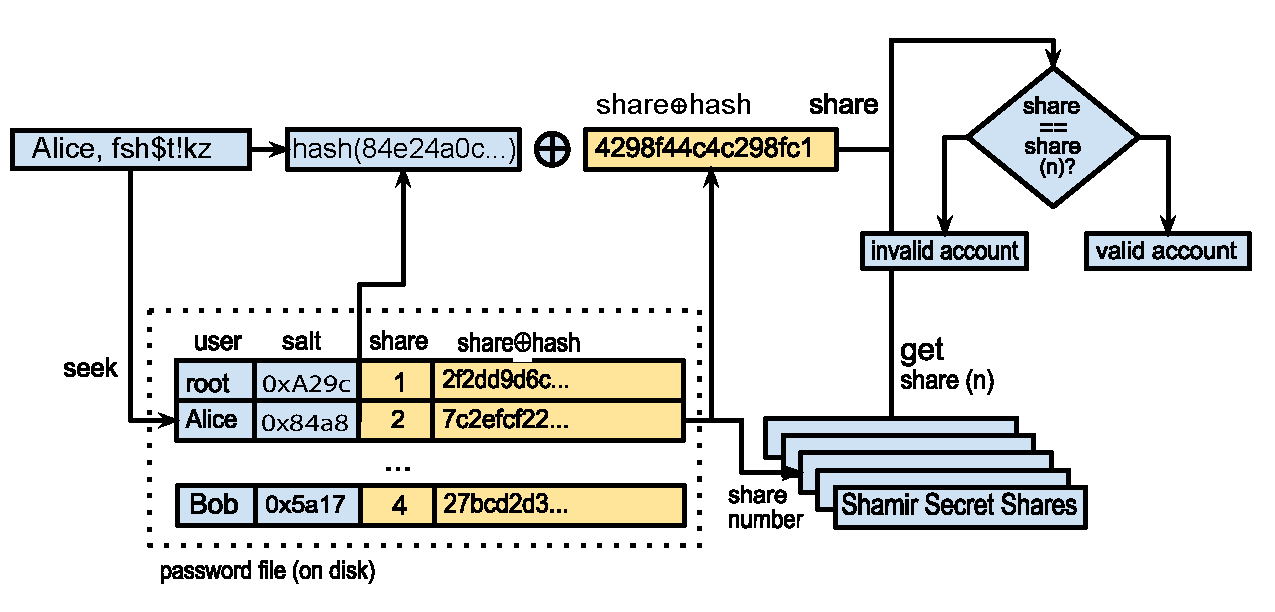
\includegraphics[width=1\linewidth]{./images/Verify_account.pdf}
    \caption{Account verification. }
    \label{FIGURE:account-verification}
\end{figure}


When prompted to validate a password, the server XORs the salted hash with the
stored data and determines whether the result is a valid share of the threshold
%cryptosystem.  For example, in Figure~\ref{FIGURE:basic-pph-algorithm}, Bob
cryptosystem.  For example, in Figure~\ref{FIGURE:account-verification}, Alice
has provided her password (`fsh\$t!kz') and the username `Alice'.  
The server and computes the salted hash of her password (`4298f44d...') and
reconstructs Alice's share (`3e773b6f...') using her share number
(2).  The server XORs the share and Alice's salted password hash together
and compares them to the value stored in the \sxh field in the password
database (`7cefcf22...').  If they match, then the password
provided was correct.

Account creation involves creating a share and XORing it with
the salted hash of the password before storing it on disk 
For example, in Figure~\ref{FIGURE:basic-pph-algorithm}, Bob registers an
account with his password (`Tr4mP0l1ne') and username (`Bob').  The 
server computes a salt (`0x5a17') and the salted hash of Bob's
password (`4153f0aa...').  The server knows the secret and knows Bob's
share number, 4. It computes Bob's share (`66ef2279...') and this value is XORed
with Bob's password’s salted hash; that value is compared to the value
stored in the database (`27bcd2d3...'). If these match, then the password
provided was correct.
%cryptosystem.  For example, in Figure~\ref{FIGURE:basic-pph-algorithm}, Bob

\begin{figure}
    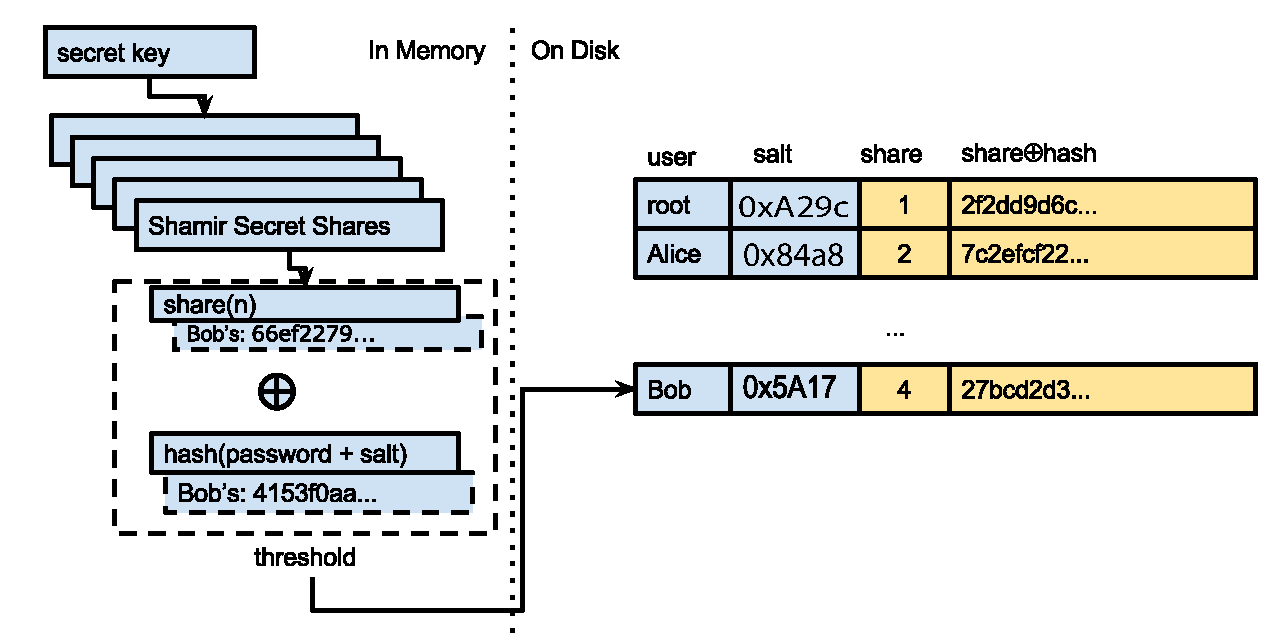
\includegraphics[width=1\linewidth]{./images/basic-pph-algorithm.pdf}
    \caption{The basic PolyPasswordHasher algorithm showing how an entry is created}
    \label{FIGURE:basic-pph-algorithm}
\end{figure}

In PolyPasswordHasher, each share protects a salted hash and each salted hash
protects a share, unless a threshold of shares is known (as is shown in
Figure~\ref{FIGURE:pph-interdependency-2}).  Suppose that an attacker has
obtained the password database and knows some set of account passwords (x,y,z).
For each known password, (illustrated in Figure~\ref{FIGURE:pph-interdependency-new}) 
the hacker can compute the salted hash and XOR this with the database entry to 
obtain the corresponding share.  If the attacker does not have a threshold of shares, 
the attacker cannot generate a share for another account (e.g., `share a').  As a 
result, the attacker cannot access share a's password's salted hash and cannot crack 
a's password.  Or, suppose that a server has a threshold of correct passwords.  
The server now has enough information to validate a threshold of shares and can use those to
recover the secret. The server could then reconstruct any share and thus,
recover the salted hash for any account's password -- an important step in
validating passwords.  Because shares protect passwords, an attacker who does
not have an adequate number of correct passwords (and thus shares) cannot
feasibly crack passwords individually. 

\begin{figure}
    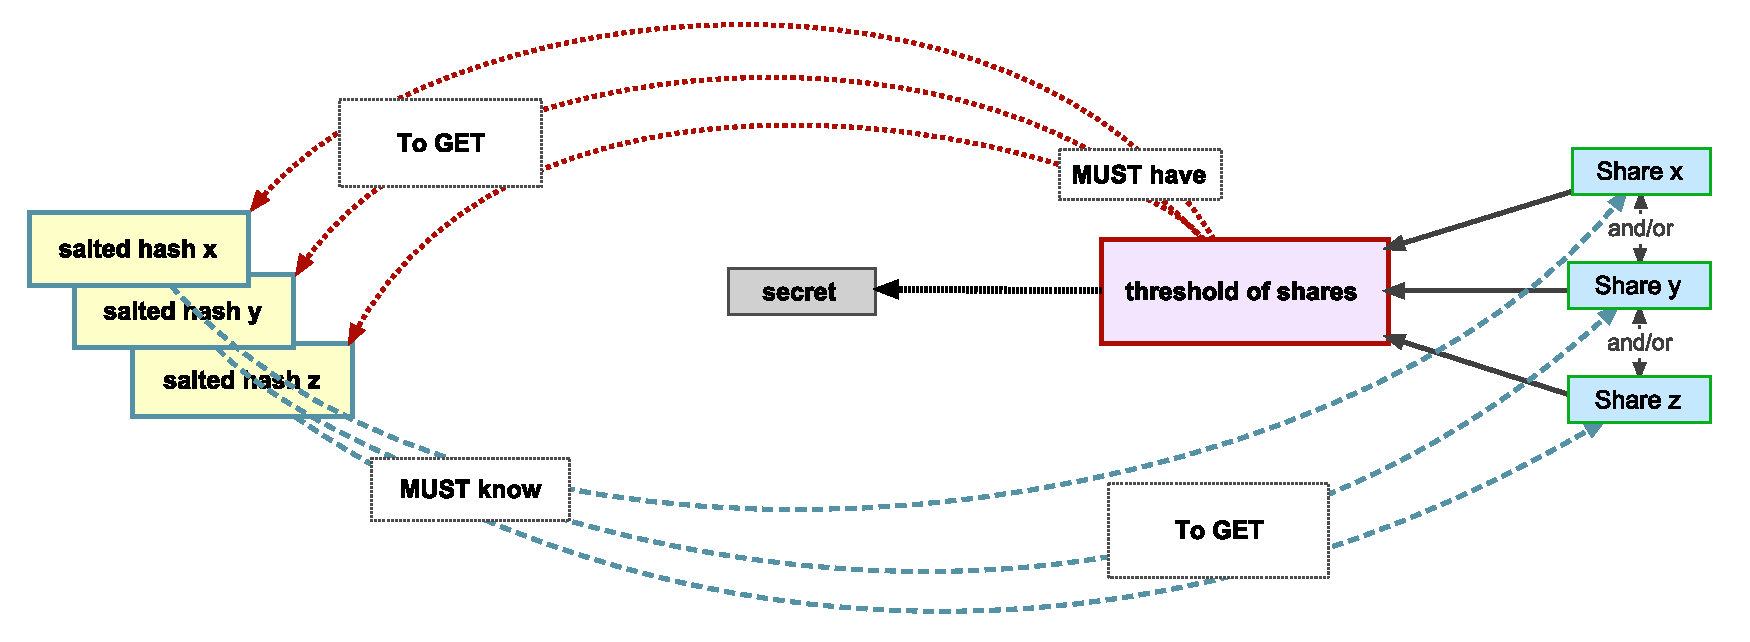
\includegraphics[width=1\linewidth]{./images/pph-interdependency-2.pdf}
    \caption{An attacker: (1) Cannot obtain salted hashes (needed to crack
    passwords) without a threshold  of shares AND (2) Cannot obtain a share without
    knowing the salted hash (password) for a \thresholdaccount.}
    \label{FIGURE:pph-interdependency-2}
\end{figure}

\begin{figure*}
    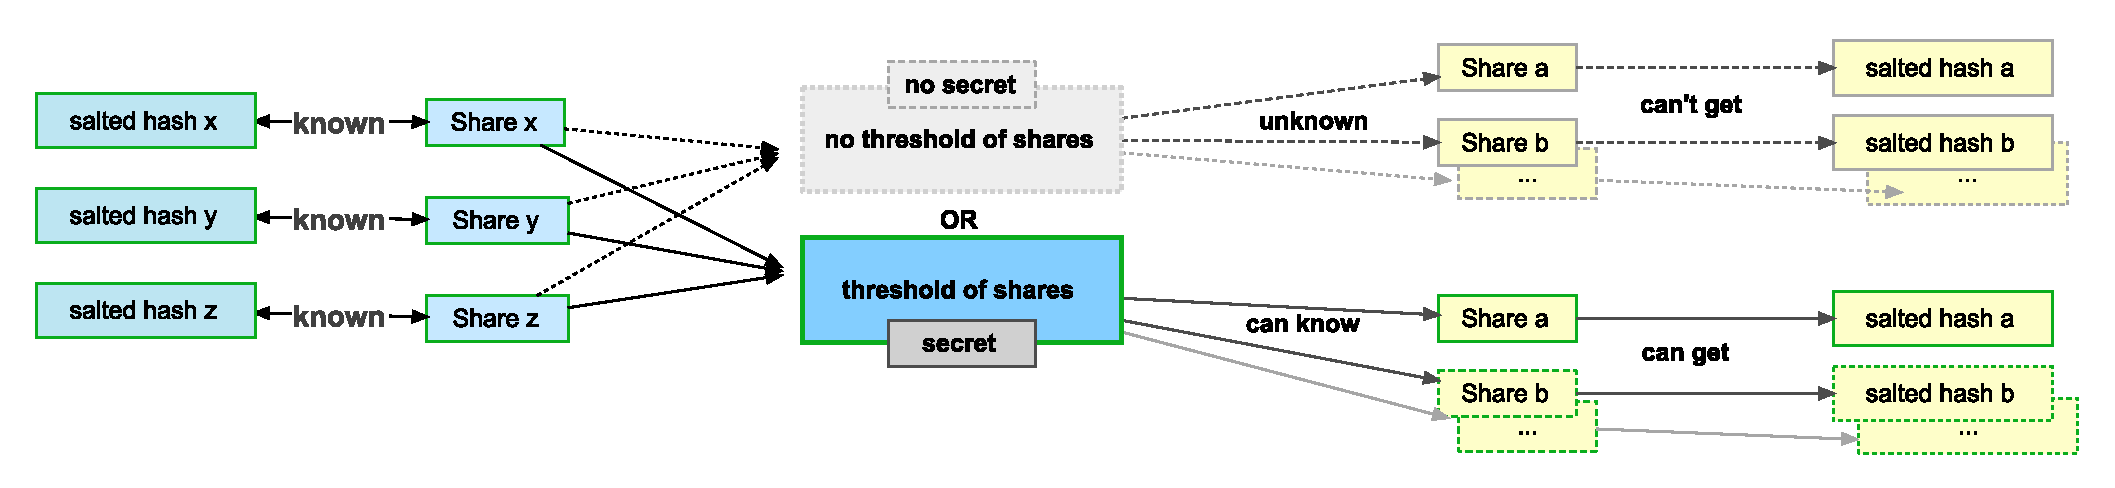
\includegraphics[width=1\linewidth]{./images/pph-interdependency-new.pdf}
    \caption{If an attacker knows some number of shares he can get the
    corresponding salted hashes; if he knows the salted hashes, he can get the
    corresponding shares; and, if he has a threshold of these, he can get the
    secret.}
    \label{FIGURE:pph-interdependency-new}
\end{figure*}
    
The basic scheme, as outlined so far, covers PolyPasswordHasher’s core 
functions.  In the remaining subsections we address how \PPH checks passwords 
without having a threshold of correct passwords (such as after a restart) and 
how it ensures that all
accounts, even those that could be created by an attacker, are protected.  To
more fully describe the full \PPH algorithm, we begin, in
Section~\ref{SUBSEC:normal-operation}, with how PolyPasswordHasher functions in
situations where the server has already validated a threshold of correct
passwords and how, after reaching this threshold, the server proceeds to login
normal users, in a phase we call normal operation.  Following this,
Section~\ref{SUBSEC:bootstrapping} discusses how \PPH performs differently when
a threshold of correct passwords have not yet been provided and needs to
acquire that threshold (e.g. after a reboot).
Section~\ref{SUBSEC:bootstrap-transitioning} discusses how the system
transitions between bootstrapping and normal operation and in
Section~\ref{SUBSEC:handling-rare-events}, we describe how unlikely situations,
such as the loss of a large number of account passwords, are handled.

\subsection{Normal operation of PolyPasswordHasher}
\label{SUBSEC:normal-operation}

Given that a server with a threshold of shares can effectively recover any
salted hash, if every account protected a share, every password would play an
important role in protecting the security of the database.  However, not all
accounts should necessarily be trusted to protect shares.  For example, a forum
may allow any user to register an account and any party, including an attacker,
to register any number of user accounts.  If these accounts each protected a
share, an attacker could easily crack the password database.

PolyPasswordHasher enables one group of passwords, which we call protector
accounts, to protect the remaining passwords in the password database; these we
call \thresholdlessaccounts.  Bob's account (who we started following in the
previous example) is an example of a \thresholdaccount
(Figure~\ref{FIGURE:protected-protector}).  An administrator will define a
threshold value of \thresholdaccounts so that if an attacker does not know a
threshold of protector passwords, Bob's salted hash cannot be recovered.  Bob's
password hash protects his share and in turn, Bob's share helps to protect the
other shares (such as shares 1,2), which in turn protect their corresponding
password hashes (for root and Alice). These shares serves to protect the full
password database, including \thresholdlessaccounts (Trudy and Luke). 

\begin{figure}
    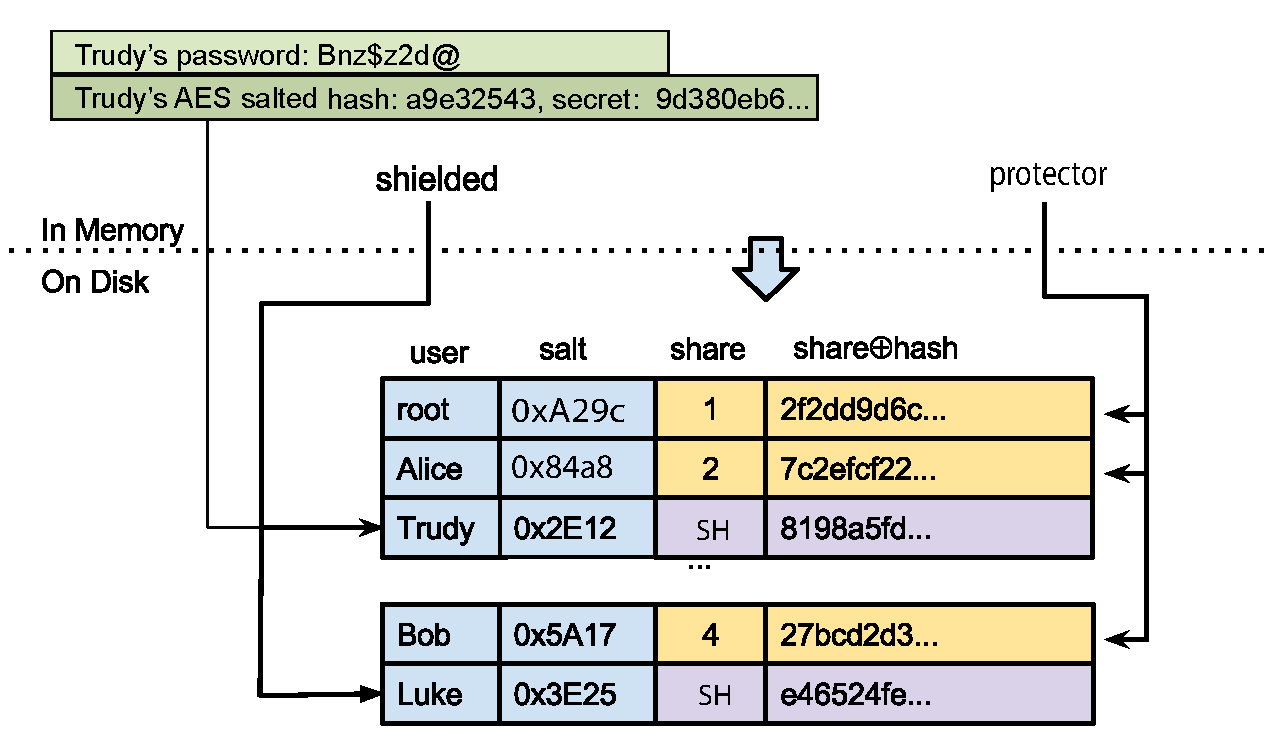
\includegraphics[width=1\linewidth]{./images/pph-store.pdf}
    \caption{A PolyPasswordHasher store with protector and \thresholdlessaccounts. \Thresholdlessaccounts are displayed with a share number of SH. }
    \label{FIGURE:protected-protector}
\end{figure}

Since a \thresholdlessaccount  does not protect a share, it is not XORed with one.
Nonetheless, these accounts are still protected by shares, or more precisely,
the secret.  \PPH uses the secret as an encryption key and with it, encrypts the
password's salted hash.  For these accounts, the resulting value (but not the
secret or salted hash) is stored in the password database.  For example, in
Figure~\ref{FIGURE:protected-protector}, Trudy's password hash (a9e32543...) is
encrypted using the secret (9d380eb6...); the result (8198a5fd...) is stored in the
database.  There are two important points to note.  First, if an attacker knows
another \thresholdlessaccount's password (e.g., Luke's), this does not
substantially help with cracking Trudy's password.  The attacker would need to
break the symmetric encryption algorithm.  Also, knowing Luke's
password would not substantially help the attacker crack the secret or other
shares in the password.  Once again, the attacker would need to break the
symmetric encryption algorithm.  Thus, \thresholdlessaccounts cannot be
effectively cracked unless an attacker knows a threshold of \thresholdaccount 
passwords.

\subsubsection{PolyPasswordHasher's algorithm}
\label{SUBSUBSEC:pph-algorithm}

Algorithm~\ref{ALG:acc-creation} details the processes of creating a user 
accounts.  The relevant operations for normal operation (lines 2-13)
are discussed in this section.  Bootstrapping operations (lines 14-23) are
deferred to the next section.

\begin{algorithm}
\footnotesize
\begin{algorithmic}[1]\Function{createAccount}{username, salt, saltedPasswordHash, isProtectorAccount}
    \vspace{.1cm}
    \State \codecomment{\footnotesize// check whether we are under normal operation}

    \If{normalOperation} \codecomment{\footnotesize// Section \ref{SEC:design} and 
    \ref{SUBSEC:normal-operation}}

        \If{isProtectorAccount} 

            \State \codecomment{\footnotesize// Obtain a share from the share cryptosystem}
            \State shareNumber, share = SecretShares.getShare()
            
            \State \codecomment{\footnotesize// Combine the share with the hash}
            \State passwordEntry = share $\oplus$ saltedHash
            \State shareID = shareNumber

        \vspace{.11cm}
        \Else~\codecomment{\footnotesize// Shielded Account 
        (Section~\ref{SUBSEC:normal-operation})}
            \State Key = SecretShares.getSecret() 
            \State passwordEntry = AES.encrypt(saltedPasswordHash, Key)
            \State shareID = \THRESHOLDLESS
        \EndIf

    \vspace{.1cm}
    \Else~\codecomment{\footnotesize// Bootstrapping (Section~\ref{SUBSEC:bootstrapping})}

        \If{isProtectorAccount}
            \State raise AccountCreationError
        \Else
            \State shareID = BOOTSTRAP
        \EndIf 
        \State passwordEntry = saltedPasswordHash
    \EndIf

    \State \codecomment{\footnotesize// Isolated Validation (Section~\ref{SUBSEC:bootstrapping})}
    \State isolatedCheckBits = saltedPasswordHash.getSuffix(IC\_BITS)
    \State passwordEntry += isolatedCheckBits 

    \State store (username, salt, shareID, passwordEntry)
    \EndFunction

\end{algorithmic}
\caption{\small Account creation pseudocode.
\label{ALG:acc-creation}}
\end{algorithm}

{\bf Creating Accounts}.  Adding an account works as is shown in
Algorithm~\ref{ALG:acc-creation}.  As the algorithm describes, the username,
salt, the password’s salted hash, and a boolean are used to indicate whether or
not the account should be a \thresholdaccount. If the account is a
\thresholdaccount, an unused share is found (line 6) and the salted hash is
XORed with it (line 8) before the share number and resulting value are stored
(line 23).  

Since a \thresholdlessaccount does not protect a share, those accounts are
instead encrypted with the secret (lines 11-12).  The share field is set to a
special value that indicates a \thresholdlessaccount (line 13).  As before,
this information is then stored in the database (line 23).
 
It is important to prevent users, particularly \thresholdaccounts, from using bad
passwords.  Similar to many deployed systems, PolyPasswordHasher employs simple
techniques to weed out extremely bad passwords.  When creating an account,
users input a password they want to use, but \PPH checks this password to ensure
that it is not too weak (e.g., ``letmein'' or ``password'').  This is done by
checking the requested password against a list of commonly used passwords (the
64K most popular). The proposed password will be rejected if it is on
that list.  PolyPasswordHasher also enforces constraints on the password length
and composition (number of lowercase and uppercase letters, numbers, and
symbols).  The purpose is not to ensure that passwords are immensely strong,
but to prevent the use of \thresholdaccount  passwords that are trivial to
guess.  These constraints are already common in many systems, such as those
that aim to prevent passwords from being cracked by brute force over the
network.  


{\bf Process for Verifying Passwords}. Assuming that the server holds the
right number of valid passwords (and thus shares), it will be able to recover
the remaining shares, as shown in Algorithm~\ref{ALG:acc-verification}.
To verify a \thresholdaccount  (lines 4-5), the server first computes the salted
hash of the user’s password and XORs it with the passwordEntry. If the
passwordEntry XORed with the salted hash is the share, then the password is
correct.  

For a \thresholdlessaccount, password verification differs because the salted hash
is encrypted instead of being XORed with a share.  Lines 8-10 of
Algorithm~\ref{ALG:acc-verification} describe how to compare the provided password
hash.  The password hash is encrypted with the secret and, if the encrypted
value matches the \sxh field, the correct password was provided.  




\begin{algorithm}
\footnotesize
\begin{algorithmic}[1]\Function{verifyAccount}{username, saltedPasswordHash, shareID, passwordEntry}

    \If{normalOperation}
        \If{isProtector(shareID)}\codecomment{\footnotesize // Section~\ref{SEC:design}}
            \State share = passwordHash $\oplus$ passwordEntry 
            \State return SecretShares.computeShare(shareID) == share
        \Else \codecomment{\footnotesize// \thresholdlessaccount , 
    Section~\ref{SUBSEC:normal-operation}}

            \State \codecomment{\footnotesize// Encrypt the obtained hash and compare}
            \State Key = SecretShares.getSecret()
            \State encryptedHash = AES.encrypt(passwordHash, Key)
            \State return passwordEntry == encryptedHash

        \EndIf
        \vspace{.1cm}

    \Else \codecomment{\footnotesize// Bootstrapping, Section~\ref{SUBSEC:bootstrapping}}

        \State \codecomment{\footnotesize// verify account created during bootstrap}
        \If{shareID == BOOTSTRAP}
            \State return passwordHash == passwordEntry
        \EndIf 

        \If{not passwordHash.endsWith(isolatedCheckBits)}
            \State return False
        \EndIf 
        \If{isProtector(shareID)}
            \State share = passwordHash $\oplus$ passwordEntry
            \State SecretShares.cacheShare(share)
        \EndIf
        \State return True

    \EndIf

    \EndFunction
\end{algorithmic}
\caption{\small Account verification pseudocode.\label{ALG:acc-verification}}
\end{algorithm}

{\bf Changing a user's password / password recovery} Changing a password
is a similar process to that used in a salted hash system, for both \thresholdaccounts
and \thresholdlessaccounts. Similar to existing systems, the procedure for
changing a password may require validating the existing password before
allowing a replacement to be generated. Changing the password involves creating
a new entry with the same username and share number. (This is nearly identical
to account creation.)  A new salt is generated and hashed along with the new
password.  Since the hash has changed, the fourth field will also change. Once
the new password entry is computed, it replaces the original stored data.  The
user may then log in normally with their new account.

\subsection{Bootstrapping After a Reboot}
\label{SUBSEC:bootstrapping}

When a system restarts, \PPH cannot validate or create accounts as it normally
would, because a threshold of valid accounts has not been reached. Because \PPH
stores shares in memory, not on disk, these are lost during reboot.  This means
that a server does not know the secret and cannot compute arbitrary shares.  As
a result, when bootstrapping, neither \thresholdaccount nor \thresholdlessaccounts 
may be verified or created using the methods described above; account creation and verification
procedures are different when the system is bootstrapping.  

%\begin{figure}
%    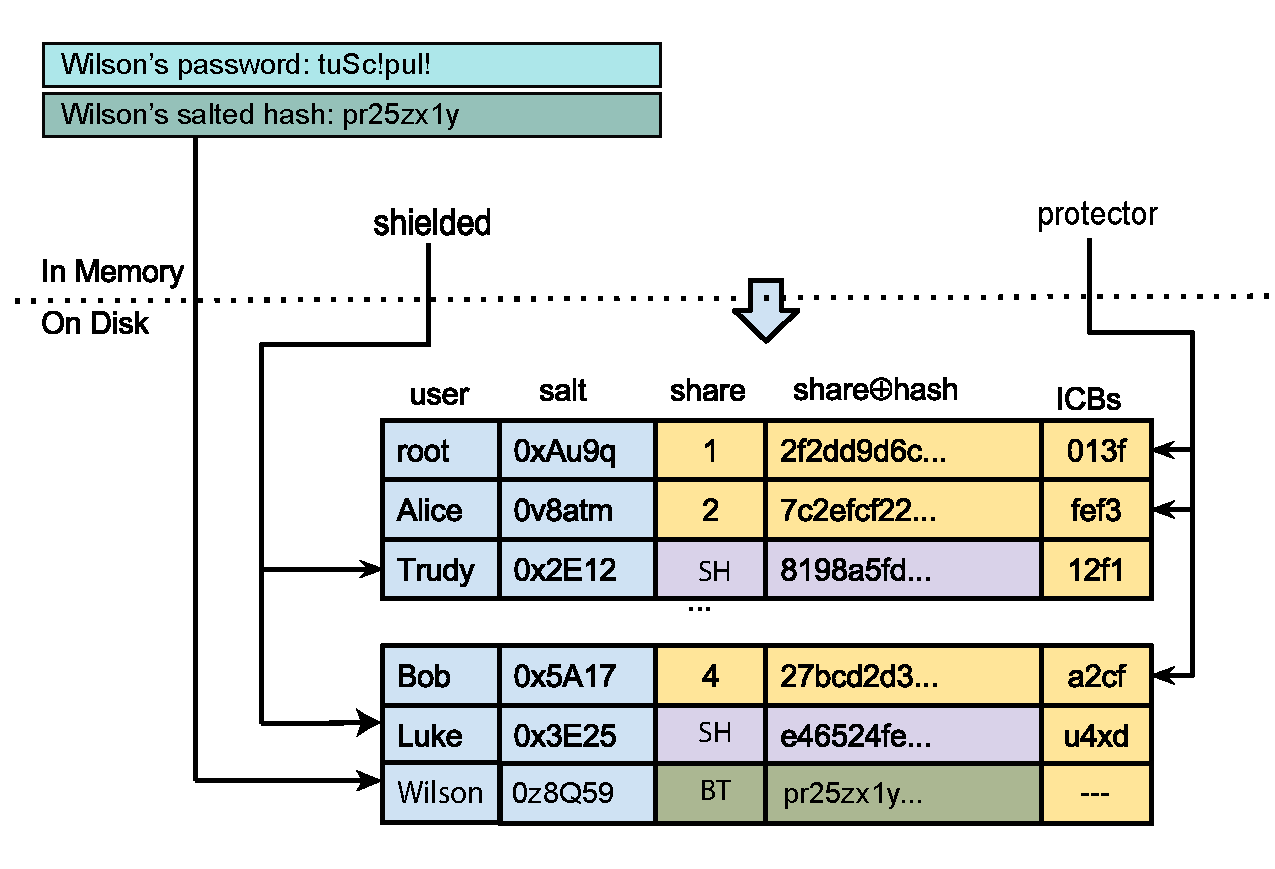
\includegraphics[width=1\linewidth]{./images/bootstrap}
%    \caption{Bootstrapping is similar to verifying an account except that we
%    use the obtained shares to restore the secret and interpolate the rest of the
%    shares.}
%    \label{FIGURE:bootstrap}
%\end{figure}

\subsubsection{Bootstrap account creation}
\label{SUBSUBSEC:bootstrap-account}

New accounts may also be created during bootstrapping. To do this, the new
account is added to the database along with the salted hash.  While the system
is bootstrapping, the new account is available to use.  In the interim, these
passwords will be created (line 19 of Algorithm~\ref{ALG:acc-creation}) and
validated (lines 18-19 of Algorithm~\ref{ALG:acc-verification}) in the same
manner as passwords stored in a system that uses salted hashes.

Although it would be easy to support \thresholdaccount creation during
bootstrap, PolyPasswordHasher does not do so (line 16 of
Algorithm~\ref{ALG:acc-creation}).  The reason is that an attacker who can
read the password database would also be able to read the salted password hash.
If the attacker can later read the password database during normal operation,
the attacker could use that salted password hash to recover the share. 

\subsubsection{Isolated Validation}
\label{SUBSUBSEC:isolated-validation}

When started, a \PPH system does not have enough protector passwords (and thus,
shares) to recover the secret.  At this point it is not possible to validate
accounts following the same process as \PPH's normal operation
(\ref{SUBSEC:normal-operation}).  Here we describe how \partialverification  can
be used to check logins even without the secret.  \Partialverification is a
process that leaks a configurable number of bits of the salted hash by using a
slow hash algorithm.  It implements a mechanism wherein it is possible, but
extremely unlikely, that an attacker could access an account using an incorrect
password.  In the next section we discuss the \partialverification mechanism,
but defer discussion of its algorithm until
Section~\ref{SUBSEC:security-properties}.

As it bootstraps, \PPH collects shares from protector logins. The number of
logins required to recover the secret will have been configured by the system
administrator, with the threshold normally set to a low number (e.g., three). 
Once the threshold has been reached, \PPH will finish bootstrapping
(Section~\ref{SUBSEC:bootstrapping}). Meanwhile, before this threshold is
reached, \partialverification makes use of an isolated-check bits field to authenticate
user passwords. 

In this scheme, illustrated in the upper right corner of
Figure~\ref{FIGURE:isolated-verification}, the password database contains
isolated-check bits.  These bits are used to verify logins before a threshold
is reached and the same process is used for both protector and shielded
accounts.  The user's password is hashed using the \partialverification hash
function.  This function returns a small number of bits of the hash (such as 24
bits of a SHA256 hash) and typically involves many iterations of a secure hash
function.  If the isolated-check bits field of the password database match the
\partialverification  hash function’s output (line 12 of
Algorithm~\ref{ALG:acc-verification}), the user is allowed to log in.

\begin{figure}
    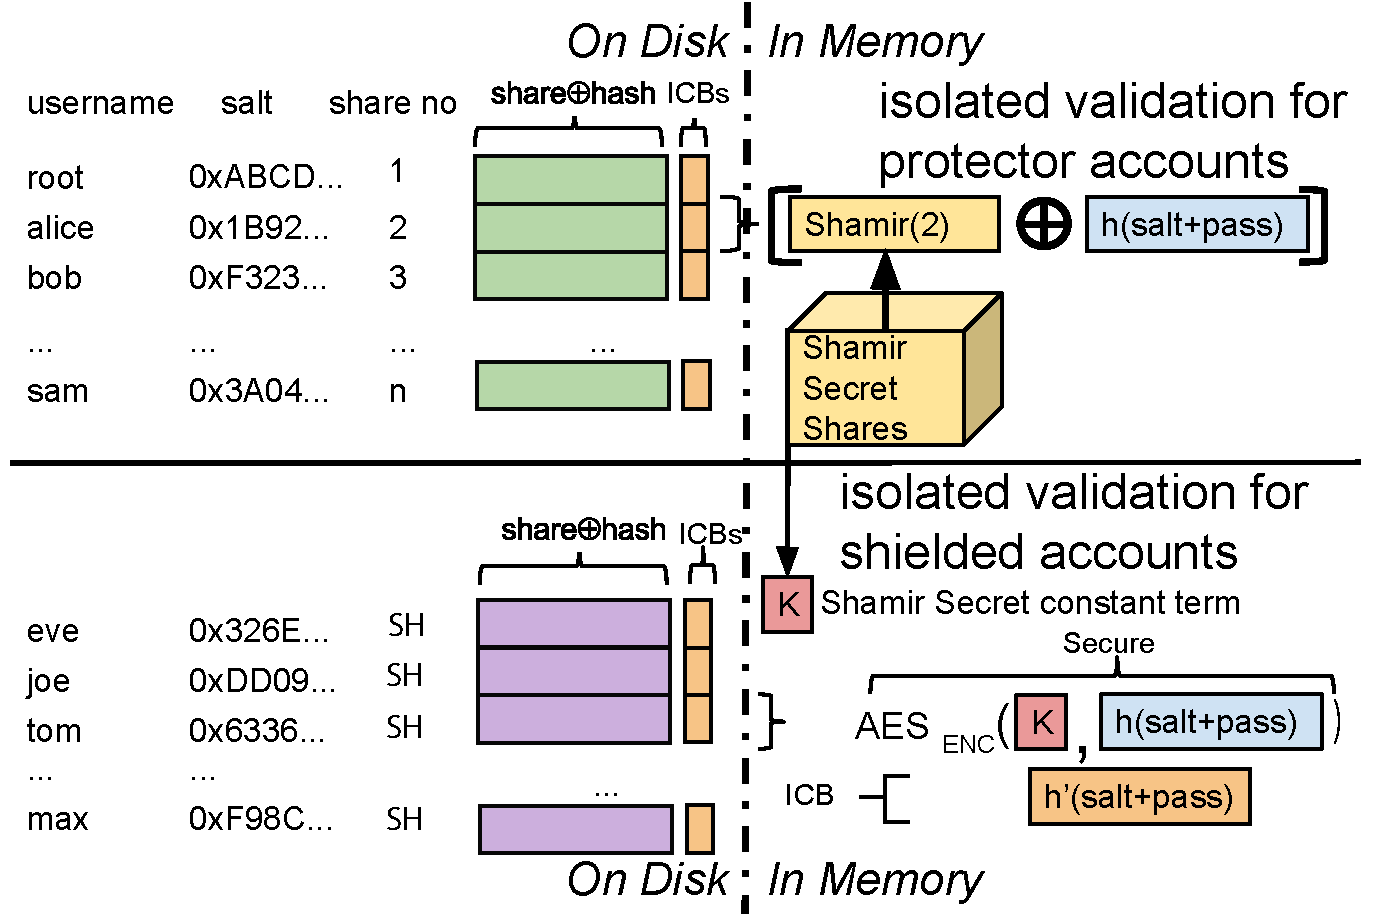
\includegraphics[width=1\linewidth]{./images/pph-with-partial-bytes.pdf}
    \caption{This figure shows validation using \partialverification. The
    isolated-check bits are stored on disk. This allows verification of accounts
    before a threshold of correct passwords is provided.  } 
    \label{FIGURE:isolated-verification}
\end{figure}

\begin{figure}
    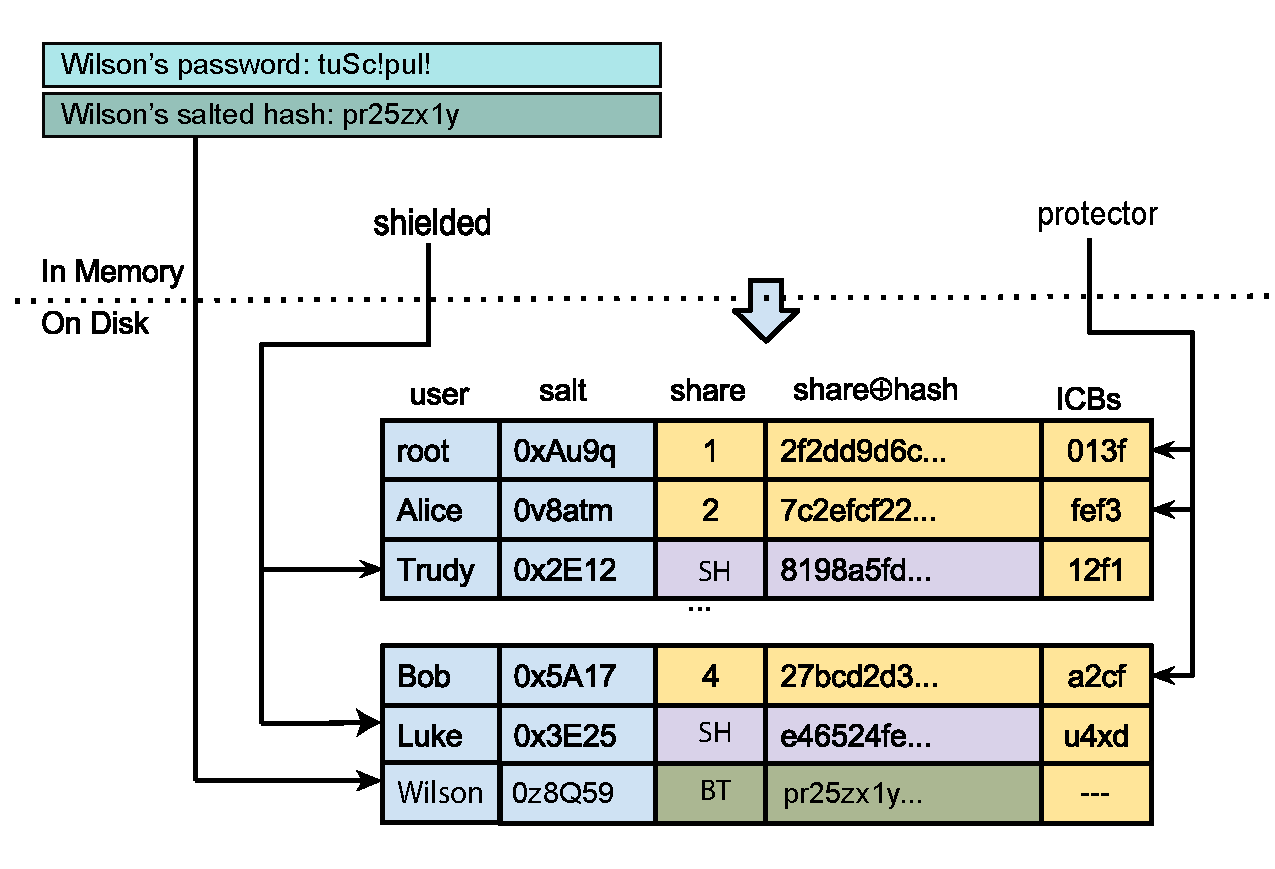
\includegraphics[width=1\linewidth]{./images/bootstrap.pdf}
    \caption{Wilson's account was created during bootstrap, so a regular
    salted hash is stored instead.} 
        \label{FIGURE:bootstrap-verification}
\end{figure}

For example, Figure~\ref{FIGURE:bootstrap-verification} illustrates 
verification while the system is bootstrapping.  Bootstrap accounts, such
as Wilson's account are validated in an identical way to a salted hash
system.  Wilson's password is salted and hashed and this is compared
with the value stored in the database.  If it matches, Wilson is logged in.

\Thresholdaccounts and \thresholdlessaccounts, like those of Trudy or Alice may
also log in while the system is bootstrapping
(Figure~\ref{FIGURE:bootstrap-verification}) using \partialverification.  The
\partialverification hash function is computed over the provided password and
the \partialbytes field is checked.  If these values match, the user is allowed
to log in. Bootstrap accounts, such as Wilson's account are validated in an
identical way to a salted hash system.  Wilson's password is salted and hashed
and this is compared with the value stored in the database.  If it matches,
Wilson is logged in.

\Partialverification represents a tradeoff for administrators.  Using 
\partialverification makes the system available immediately after a reboot.  
However, when using a small number of \partialbytes, there is the potential
for an incorrect authentication during the bootstrapping phase.  Alternatively
a large number of \partialbytes impacts the confidentiality of the password
database in the event of a theft, by making the passwords easier to crack.
Thus in some scenarios different settings are appropriate, possibly
even for \thresholdaccounts and \thresholdlessaccounts in the same database.
We explore this tradeoff more in Section~\ref{SUBSEC:security-properties}

\subsection{Transitioning From Bootstraping to Normal Operation}
\label{SUBSEC:bootstrap-transitioning}

As the system bootstraps, the server batches shares from \thresholdaccounts
(line 14 of Algorithm~\ref{ALG:acc-verification}).   After the system has a
threshold of shares, it is possible to recover the secret. The server performs
Lagrange interpolation, which allows the server to not only recover the secret
but also, to generate arbitrary shares (both are needed to check \thresholdlessaccounts).  

Recall that accounts created during the bootstrap phase contain BOOTSTRAP for
their share number and have a salted hash stored in the database.  When the
system recovers the secret and transitions to normal operation, these accounts
will have their password hashes encrypted with the secret and their share
number field set to \THRESHOLDLESS.  This transforms these accounts to the same
state as \thresholdlessaccounts that are created in normal operation.

Also, all account logins that were processed during bootstrapping are now
checked to be certain that the correct passwords were provided.  This step is
needed because it is possible that an attacker could find a password that is
invalid and yet, matches the \partialbytes.  (We examine the feasibility and
computational cost of this in Section~\ref{SEC:evaluation})  The salted
password hash for \thresholdlessaccount logins are cached in memory and the
passwords are verified once a threshold is reached.

For a \thresholdaccount , if a provided password hash matches the \partialbytes,
but the password is not correct, the recovered share is not invalid.  The
incorrect share will be detected when a threshold of shares are obtained
because the integrity check on the secret will fail.  If this integrity check
fails, the administrator is notified.  The system can still enter normal
operation once a threshold of valid shares are obtained.  

\subsection{Handling Rare Events}
\label{SUBSEC:handling-rare-events}

At an administrator's behest, accounts may be switched between shielded
and protector without user intervention. To do this, the server must be in
normal operation.  The server can then recover the salted secure hash. This
salted secure hash can then be re-encoded (using a share for an account that
becomes a \thresholdaccount; or encrypted, for an account that becomes
shielded) and the new entry can be stored. This transitions the account
from a protector to shielded (or vice versa).

{\bf Recovering data if all \thresholdaccounts are lost}.  If not enough
known threshold users can be verified, the salted hashes are lost forever and
accounts cannot be validated using the technique we described in
Section~\ref{SUBSUBSEC:isolated-validation}.  However, this does not mean that
the system is unusable because \partialverification allows users to log in.
Furthermore, mechanisms like root password recovery that are done through the console
will still work, and will allow any data on the system to be accessed.

{\bf Trusting a \thresholdaccount with multiple shares}.  A single
account may optionally provide access to multiple shares. 
To do this, a single user can have multiple rows in the table.  Each 
row will have a different \sxh entry and thus protect a different share.
Each entry must also have a different salt to ensure that a different
hash value is XORed with each share.  When the user provides their password,
the value can be used to recover the share in each row by XORing the salted
password hash with each share.

{\bf Detecting an \partialbytes match of an incorrect password}.  If the
system is in normal operation, it will detect that the password does not match.
However, PolyPasswordHasher will always check the \partialbytes for an entered
password (for clarity, not depicted in Algorithm~\ref{ALG:acc-verification}).
If the password is incorrect, but the \partialbytes match, this indicates that
an attacker has almost certainly stolen the password database but has not (yet)
cracked the password.  This generates an alert to the administrator to notify
her of the likely breach.



\section{Implementation}
\label{sec-implementation}


Our reference implementation for PolyPasswordHasher is available with an MIT license 
at \showurlx.  It utilizes
a 16 byte salt, with SHA256 to compute password hashes.   The Shamir
Secret Sharing routines
utilize GF256 as the underlying field (encoding each byte as a separate
share).   %The implementation of Shamir Secret Sharing was written while
%referencing the open source Python {\tt tss} implementation, but was 
%essentially rewritten to handle the interfaces needed by PolyPasswordHasher.   
The full code base for PolyPasswordHasher is 203 lines of Python code and
223 lines of C code\footnote{
All line of code counts are according to SLOCcount~\cite{wheeler-sloccount}}.   
PolyPasswordHasher uses Python's standard hashlib for SHA256 and the PyCrypto
implementation of AES.
The GF256 operations, Lagrange interpolation, and polynomial math code
are written in C for performance reasons.   All other code is written in 
Python.  The main code for PolyPasswordHasher, which handles account
creation, accessing a persisted store, writing a store to disk,
checking passwords, and similar operations, is 87 lines of Python code.
Adding support for thresholdless accounts involved adding 20 lines of Python
code.   Partial verification added 13 lines of Python code.
The remaining Python is wrapper code for the C-based 
Shamir Secret Sharing implementation.

%\url{https://polypasswordhasher.poly.edu/}.   
%We release the code as open source 
%under an MIT license.




\section{Evaluation}
\label{SEC:evaluation}


To evaluate \PPH, we evaluated the feasibility of its use 
in different scenarios.  This includes issues ranging from the efficiency
of the algorithm, to the expected security benefits from different 
configurations and deployment scenarios.  We frame our evaluation around
the following questions:

\begin{itemize}
    \item How long does \PPH take for different operations?
    \item What is the storage cost of \PPH?
    \item How much memory is needed for \PPH?
    \item What are the security properties of \PPH?
        \begin{itemize}
            \item What happens if users pick weak passwords?
            \item What \partialbytes settings should be used?
            \item How does the threshold affect the cracking time?
            \item What if a poor value is chosen for the threshold?
%            \item What is the feasibility of an attacker cracking a \PPH
%                protected store, with strong \thresholdaccount passwords
        \end{itemize}
\end{itemize}

%We will evaluate the time, memory and storage aspects of the algorithm and our
%python reference implementation. After this, we will analyze what are the
%optimal configuration values for \PPH by studying the behavior of the algorithm
%when we vary any of its parameters. Finally, we will summarize our findings and provide a
%case study to compare \PPH with regular salted hashes.

\subsection{What is the time cost of \PPH?}
\label{SUBSEC:time-costs}

To evaluate time costs, we examined how long it took PolyPasswordHasher to
process account verifications, new accounts, password changes, initializations
of a password store, and transitioning from bootstrapping to normal operation.
We measured the processing speed and performance of \PPH using an early-2011
MacBook Pro with 4GB of RAM and a 2.3 GHz Intel Core i5 processor.  All
operations reflect the mean verification time across 100 runs and were
performed with the password file already present in memory. For benchmarking
purposes, each action was performed sequentially despite being embarrassingly
parallelizable.

Figure~\ref{FIGURE:running-times} shows the time taken by different
operations (discussed below). Unless noted, the time cost of an operation did
not depend on other factors, such as the number of accounts in the password
database.

\paragraph{Time to verify an account} The mean time to verify a
\thresholdaccount was around 60$\mu$s independent of the threshold value.
For example, a threshold of eight allowed a server to verify more than 16K user
accounts per second.  Verifying a \thresholdlessaccount took approximately 29$\mu$s
and the server processed about 35K such actions per second. Bootstrap accounts,
which use salted hashing, took just over 3$\mu$s on the same platform.

The values presented do not include key stretching.  (Except for
the case of \partialverification, key stretching is unlikely to be used
for individual account verification with \PPH.)  
%At a minimum, we need to say we assume 1 billion hashes a second, if we
%assume that~\cite{ElcomSoftGPUCracking,zonenberg2009distributed}...


\begin{figure}
    \centering
    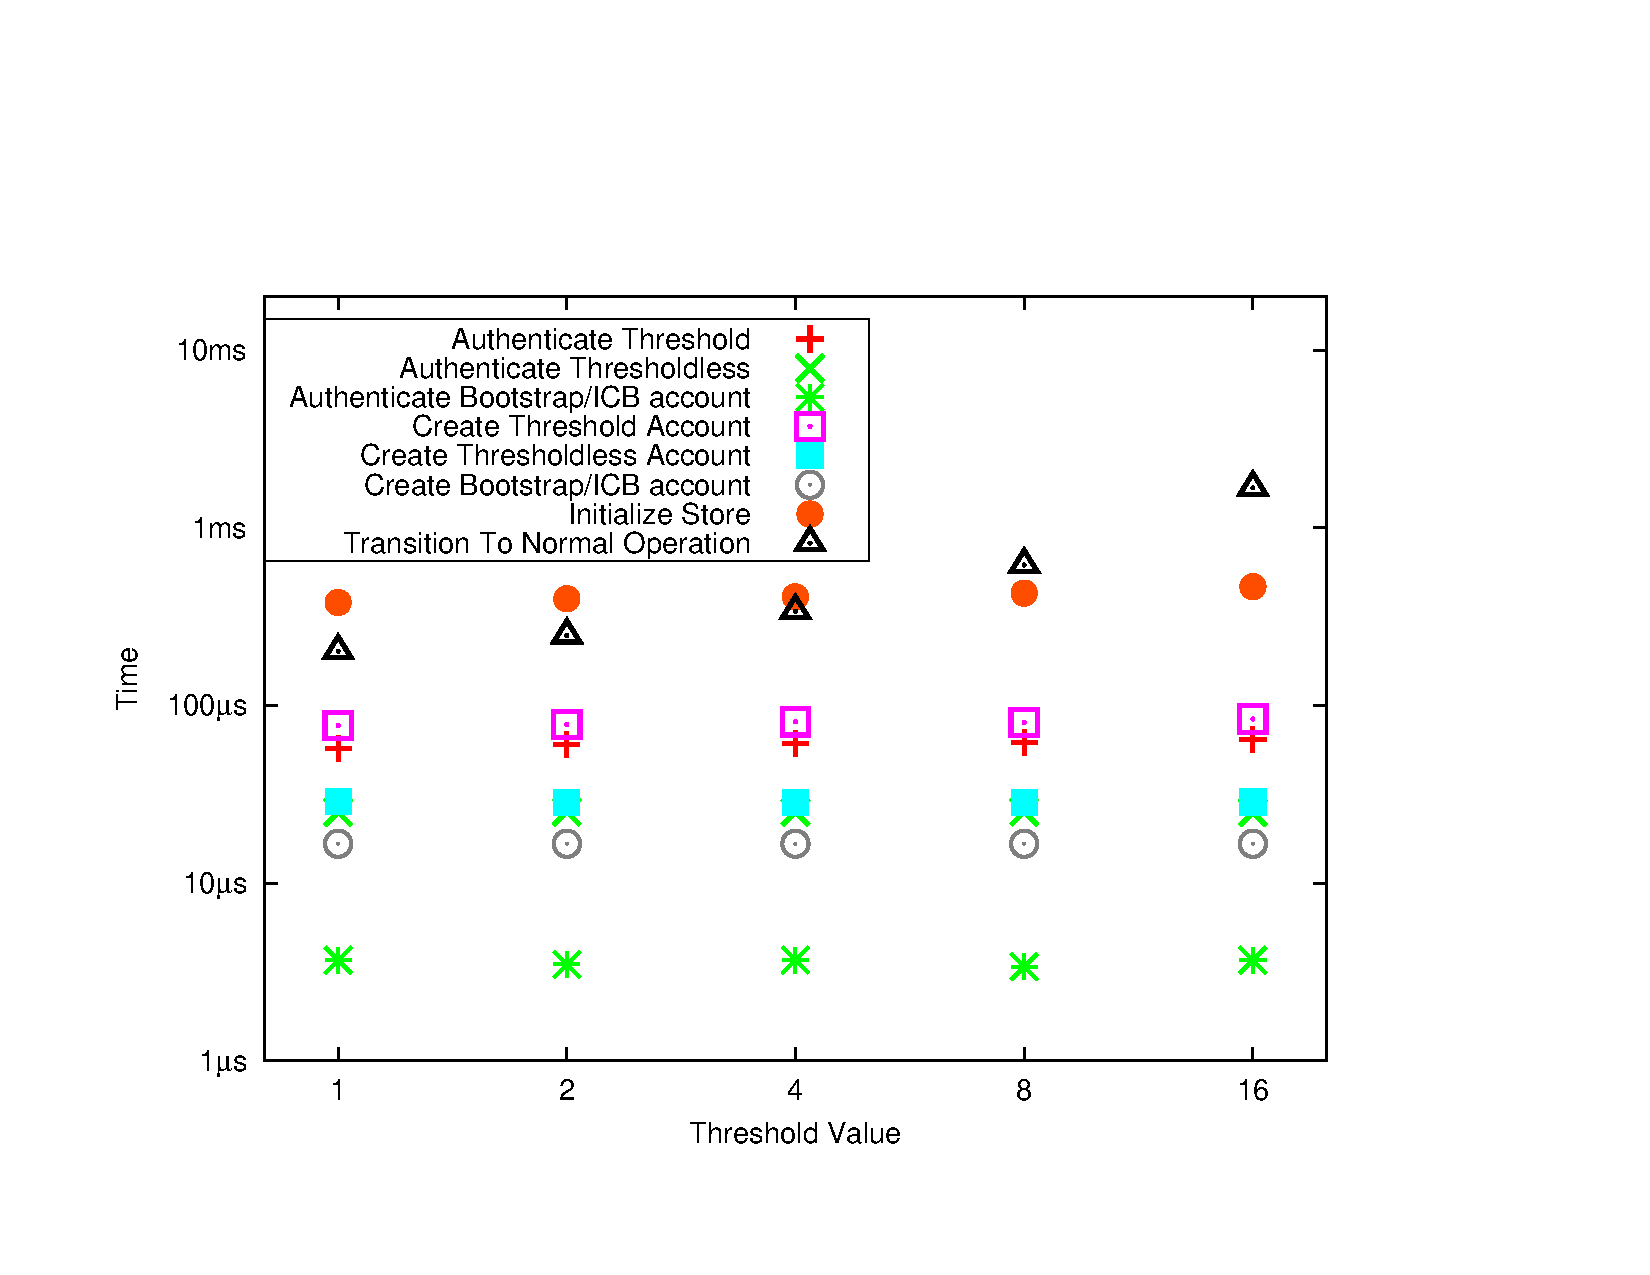
\includegraphics[width=.5\linewidth, trim=205 65 280 105]{./images/pph-running-times.pdf}
    \caption{Time needed per operations in \PPH. 
    \Partialbytes verification and transition to 
normal operation times are listed without key stretching.   }
    \label{FIGURE:running-times}
\end{figure}


\paragraph{Time to create accounts or process password changes}
Account creation time was similar to the time needed to verify accounts.
Depending on the threshold value, the average creation time varied from
77$\mu$s to 85$\mu$s. A \PPH store with a threshold value of eight created more
than 12K accounts per second. Given that there are a maximum of 255
\thresholdaccounts that can be created (at least with a \PPH implementation
that uses GF256), \thresholdaccount  creation time is not a performance
concern.  \Thresholdlessaccounts were created independent of the threshold, in
about 25$\mu$s. Based on this, we calculated that approximately 40K
thresholdless accounts can be created each second. This is similar to the time
it takes to generate a salted SHA256 hash for a password (16$\mu$s).  Changing
a password only requires \PPH to perform the same operation it uses to
create an account (and potentially also authenticate the old password).

\paragraph{Time needed to initialize a password database} The time to create a
database varied and was dependent on the threshold value used.  However,
varying the threshold from 2 to 16, varied the creation time from 380$\mu$s to
460$\mu$s. This time cost is largely due to the need to generate
cryptographically-suitable random numbers; but this operation is only
performed once, when a new password file is created.


\paragraph{Time needed to transition to normal operation} When the
server restarts, random coefficients are computed from the set of provided
shares, with full interpolation. The time needed to complete this operation
varied between 202$\mu$s and 1.6ms, because the threshold changes in relation to
changes in the number of polynomials, as the store size increases.  Note that
small thresholds were processed quickly --- a store with a threshold of 8 was
unlocked in 617$\mu$s.  There is also the time needed to do the integrity
check on the recovered secret.

Computing the random coefficients and computing the integrity
of the recovered secret (via a cryptographic hash) needs to be done once per 
restart for a normal server.  However, an attacker attempting to crack the
database will recompute the random coefficients and compute the hash once
per guess of \thresholdaccount values.  We therefore recommend that the 
integrity check use enough iterations of the hash function to increase the 
computational time needed to at least 100ms.   This slows the attacker
down per guess (a frequent operation), while only delaying the server slightly
one time per reboot.

{\bf Recommendation 1: The integrity check on the secret that is performed
when transitioning to normal operation should take at
least 100ms to complete.}

\subsection{What is the Storage Cost of \PPH?}

\begin{table}[t]
    \centering
    \renewcommand{\arraystretch}{1.3}

    \begin{tabular}{| c | c | c | c | c | c |}
    \hline
    {\bf Password } & {\bf Original} & {\bf Salted Hashes} & {\bf PPH }& {\bf PPH } & {\bf PPH }\\
    {\bf source} & {\bf space} & {\bf space} & {\bf No IV} & {\bf (16 ICB)} & {\bf (24 ICB)}\\
    \hline
    RockYou & 134MB & 260MB & 265MB & 275MB & 280MB\\
    \hline
    eHarmony* & 51.6MB & 100MB & 102MB & 106MB & 108MB\\
    \hline
    Formspring* & 27.3MB & 34.8MB & 35.2MB & 36.0 MB & 36.4MB\\
    \hline
    Gawker & 75.2MB & 119MB & 120MB & 122MB & 123MB \\
    \hline
    LinkedIn* & 252MB & 424MB & 430MB & 442MB & 448MB\\
    \hline
    Sony & 2.98MB & 4.95MB & 5.00MB & 5.10MB & 5.15MB\\
    \hline
    Yahoo & 17.8MB & 35.0MB & 35.4MB & 36.2MB & 36.6MB\\
    \hline
    \end{tabular}
    \caption{Disk space needed to store leaked password databases in
    different formats. * Denotes breaches in which only the salted hash portion
    of the database was released}
    \label{TABLE:disk-space}
\end{table}


%   ['eHarmony', 51.6, 100.0, 102.0, 104.0, 106.0, 110.0]
%   ['Formspring', 27.3, 34.8, 35.2, 35.60000000000001, 36.000000000000014, 36.80000000000002]
%   ['Gawker', 75.2, 119.0, 120.0, 121.0, 122.0, 124.0]
%   ['LinkedIn', 252.0, 424.0, 430.0, 436.0, 442.0, 454.0]
%   ['Sony', 2.98, 4.95, 5.0, 5.05, 5.1, 5.1899999999999995]
%   ['Yahoo', 17.8, 35.0, 35.4, 35.8, 36.199999999999996, 36.999999999999994]


Storing passwords with \PPH requires that additional information
-- a one byte share number -- be stored for each account.  This adds one byte
of storage space for each account, beyond the cost of current hash techniques.
The one byte has minimal impact on the disk space needed to store production
password databases (Table~\ref{TABLE:disk-space}).
% If \thresholdlessaccounts are stored in a
%separate file or are somehow distinguished stored independently, then only
%\thresholdaccounts require the extra byte of storage. This results in a cost
%for those accounts that is identical to the salted, hashed scheme. 

If the \partialbytes
field is used, the amount of information increases by the size of the field. 
For example, with a value of $24$ \partialbytes, the total cost increases by 
four bytes (one for the share number and three for the \partialbytes field). 

\subsection{How much memory is needed for \PPH?}

\PPH uses more memory than does a salted hash solution in normal operation.  
The server must store the polynomial coefficients for the 
Shamir Secret Share (which includes the secret).  However, the total size
of this data is relatively small --- the threshold value (2-5) multiplied by 
the length of the \sxh field (32 bytes).  As this value is likely to be
a few hundred bytes in practical deployments, (which is smaller than the \PPH 
code will be in memory), this should not pose a problem in practice.

During bootstrapping, additional memory is also used.  While shares are being
acquired, they are kept in memory.  This has a similar cost to storing
the polynomial coefficients for the Shamir Secret Share.
However, if \partialverification is used, the more
substantial cost is storing authentication information so that it can be
verified against the complete entry to ensure that the previous login was
correct. The memory cost of caching this information will correspond to the
number of logins before bootstrapping is finished (i.e., \sxh * Log-ins).
The total memory cost is still rather small, even for a server that processes
many authentications.  For example, a server that processes ten thousand logins
while bootstrapping needs only 320KB of memory to store that information.  Thus
the memory costs remain small, even for heavily used systems.
 


\subsection{What happens if users choose extremely weak passwords?}
\label{SUBSEC:bad-passwords}

If extremely weak passwords are
used for a threshold of \thresholdaccounts (like administrators), \PPH will not
provide strong protection.   If there are only a few bits of entropy in the
password, the search space will still be small, but exponentially larger.   
For example, if the attacker knows that three \thresholdaccounts each chose one
of 10 weak passwords, the attacker could sweep the search space in 1000
guesses (100 seconds, given a 100ms time to verify the secret).  While this
is much better than the 30 guesses an attacker would need with salted hashing,
this protection is obviously still very weak.  It
is thus critical that \thresholdaccounts are secured with strong passwords.  
\PPH performs very poorly when weak passwords are used for \thresholdaccounts.  Even 
with extremely weak passwords, \thresholdlessaccounts will have some 
protection, so long as the \thresholdaccounts use strong passwords.  

However, independent of any storage technology, extremely weak passwords 
are susceptible to guessing by an external party without having to steal
the password database.  Therefore, this is not an area that password database
storage technologies can address.

Fortunately, research has shown that users can be helped to choose passwords
that have a significant degree of randomness.  This can be done by requiring a combination of
passwords that are a certain length (8 characters), combinations
of character types (letters, numbers, symbols), and by blacklisting common
passwords~\cite{weir2010passwordpolicies}.  Extremely weak passwords are
susceptible to guessing by an external party (without database access); as
best practice, sites should block them from use~\cite{bancommonpasswords,
weir2010passwordpolicies, cormac2014telepathwords,
kelley2012guessingpasswords}.  The combination of length, diverse character
types, and blacklisting common passwords has been shown to substantially
increase the time needed to crack passwords.

%We applied these techniques to passwords from the RockYou password dump
%and then evaluated the entropy of the resulting password entries.  We 
%found ...\cappos{Continue in this vein with results...}
%Thus we expect the \thresholdaccounts can
%pick passwords with ?? bits of entropy; equivalent entropy to
%a ????-character-long, random password.


{\bf Recommendation 2: \Thresholdaccounts should have
as much entropy as a 6-character-long random password.}


%However, \PPH provides the ability to protect \thresholdlessaccounts even if they do not
%pick good passwords, for they are protected by the \thresholdaccounts. When an
%attacker attempts offline cracking on a \PPH-enabled database, his only
%alternative is to crack different \thresholdaccounts simultaneously first, and then
%crack the whole database as he would do against regular salted hashing. 


\subsection{{\bf What \partialbytes setting should be used?}}
\label{SUBSEC:security-properties}

%\cappos{Throughout the paper, we need to be sure we don't say 
%\partialbytes = 0, when we mean disabling \partialverification.  
%We never mean \partialbytes = 0.  We should always say disabling instead.}

\Partialverification changes the properties of \PPH, depending on the
size of the \partialbytes field.  
\begin{itemize}

\item When \partialverification is disabled, a user may not log in until a
threshold of \thresholdaccount passwords have been provided.  This makes \PPH
unavailable during the bootstrap phase.  

\item When the size of the \partialbytes field is very small, 
it is possible that authentication errors will be made during bootstrapping.
For example, if the size of the \partialbytes field is set to 1 bit (an
implausible and extreme example), then an attacker typing a random password 
has a 50\% chance of the \partialbytes matching and being allowed in.

\item  As the size of the \partialbytes field grows, the probability that an
attacker will succeed with online cracking decreases. However, when the size of the
\partialbytes field is very large, if an attacker steals the database, the
confidentiality benefits of \PPH are weakened.  For example, in the extreme
case that the \partialbytes field is the size of the entire salted password
hash (an implausible example), then an attacker can use the slow,
\partialverification hash to individually crack passwords.  In this case, from
a security standpoint, \PPH is effectively equivalent to key stretching.  The
primary benefit of \PPH in this case is that it does authenticate accounts much
more quickly in normal operation than does key stretching.

\end{itemize}

Given that the size of the \partialbytes field and the threshold is
configurable, the security properties of \PPH vary. When integrating \PPH into
a system, an administrator can leverage this adaptability to better meet his
expectations.  In the next subsection we explain how different configurations 
of \PPH apply to different use cases.


\begin{figure}
    \centering
    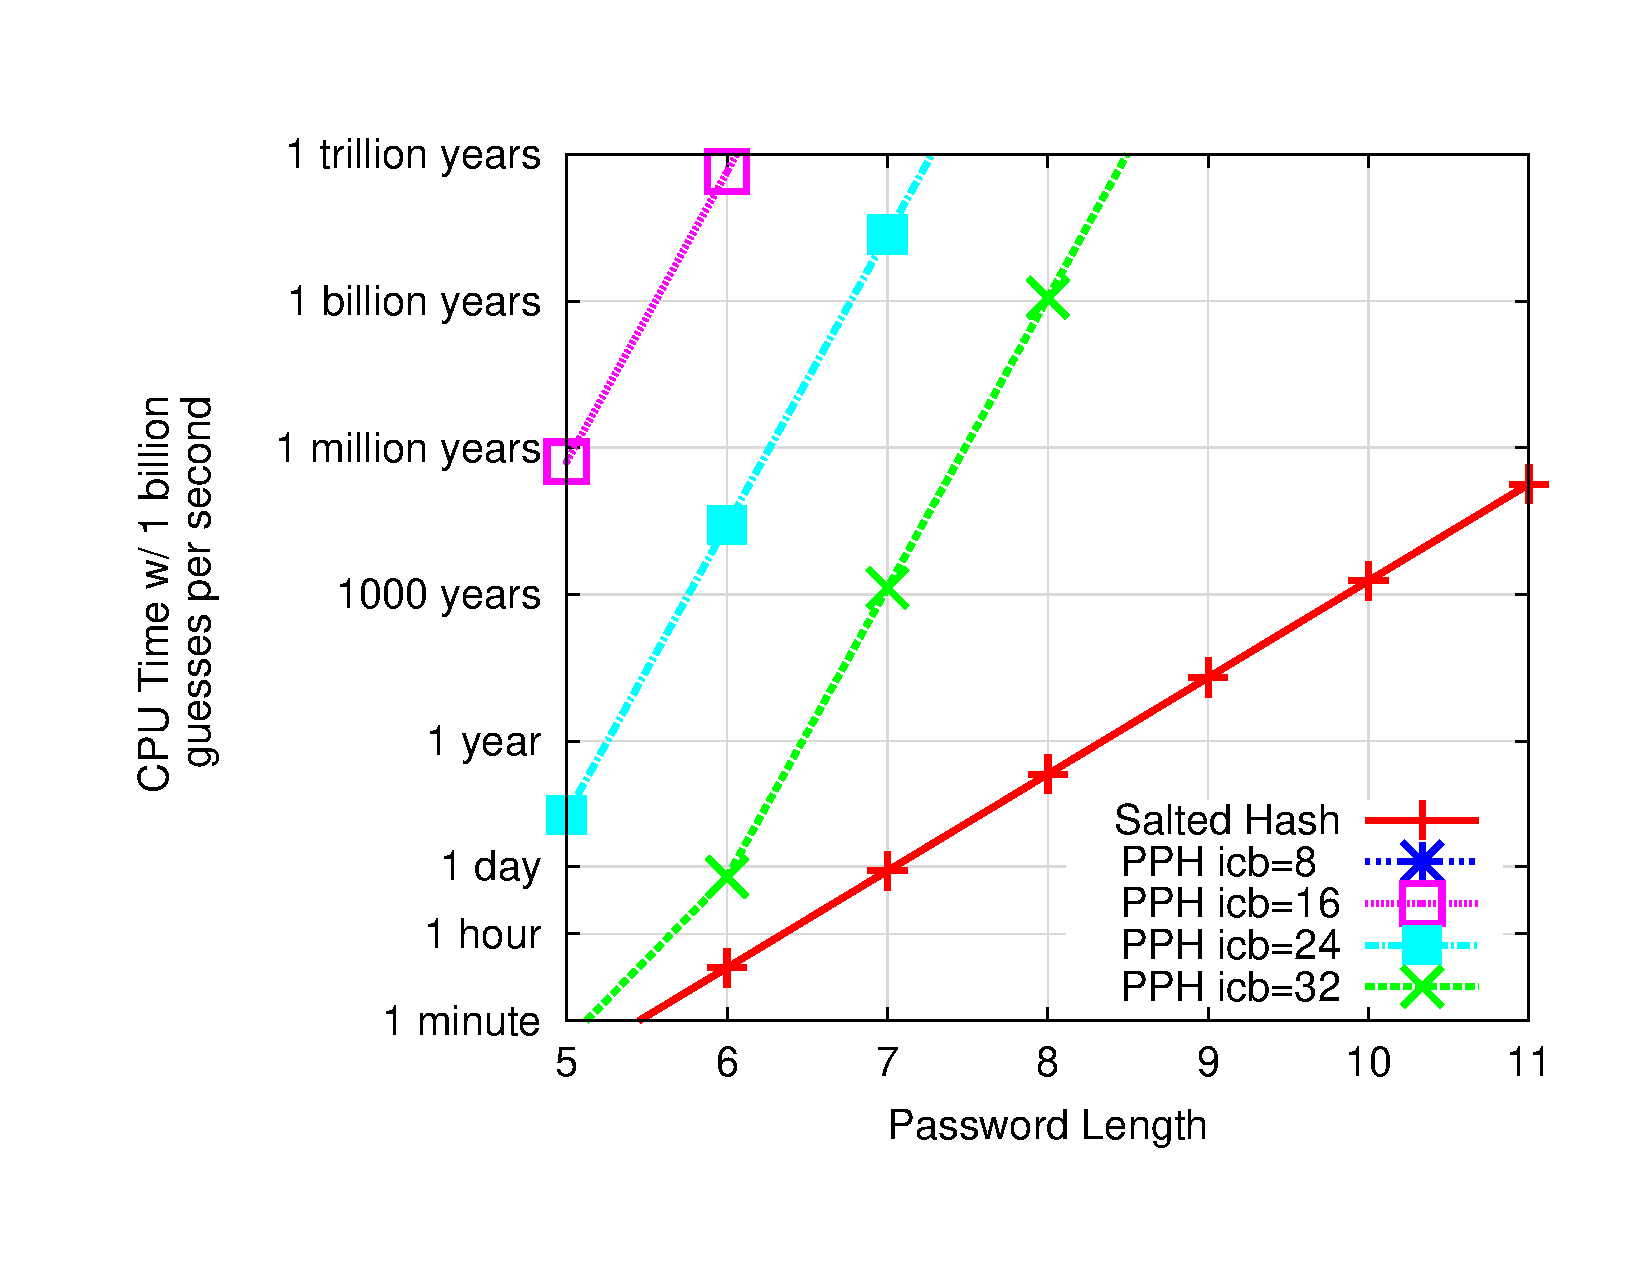
\includegraphics[width=.5\linewidth, trim=195 55 165 55]{./images/plotcrack_icb}
    \caption{{\small Time it takes to crack a \PPH store with different values
    for \partialbytes and a threshold of 3.  The line for \partialbytes=8
does not fit within the axes of the graph. }}
    \label{FIGURE:cracking-icb}
\end{figure}



\subsubsection{Immediate Availability For Many Unknown Clients}
In some situations, after
reboot a server needs to be immediately available to a potentially huge 
number of untrusted clients.  For example, a 
web forum or a social media site is likely to have this property.
Availability is paramount, for a large, diverse, and constantly changing
user base.

If an attacker has his attack detected and his IP address blocked, this 
may not be a major concern or deterrent. Therefore, attackers may try to do things such as
brute force passwords, even if this is likely to lead to detection.

There is also a risk of users trying incorrect passwords during the bootstrap
phase to try to break into an account.  Most existing web frameworks deal with
this by restricting the number of password attempts from an IP address over a
period of time (10 authentications per second is common).  However, a motivated
attacker with the ability to connect from many IP addresses (e.g., a botnet
operator), could still be able try a substantial number of passwords.
However, using a \partialbytes value of 24 bits will cause the attacker's
password search space to be as large as the usual number of attempts for
successful online cracking scenarios.

% \cappos{probably discuss somewhere here how bootstrapping is only used
% for a short time..}



The downside is that a large \partialbytes field will make it easier for an
attacker to crack the \thresholdaccounts.  As shown in
Figure~\ref{FIGURE:cracking-threshold}, as the size of the \partialbytes field
grows, the cracking time for a threshold of three starts to resemble the time
for salted hashes. For 24 \partialbytes, the time to crack a six-character
equivalent random password is around $270420$ years. In summary, the
\partialbytes setting reduces the password entropy.  To provide adequate
protection, either passwords with the entropy of 8 character random passwords
should be used, or, as will be discussed later, the threshold should be
increased.


{\bf Recommendation 3: In situations where a large number of unknown clients
will authenticate, use a setting of 24 \partialbytes.}


\subsubsection{Immediate Availability For Known Clients}
In many cases, the set of expected clients is limited and known.
This includes situations like a institutional file server or mail server.
In this case, the total set of possible clients is limited and it is
assumed that an attacker cannot control a large number of IP addresses / 
clients.

\begin{table}[t]
    \centering
    \renewcommand{\arraystretch}{1.3}

    \begin{tabular}{| c | c | c | c |}
    \hline
    {\bf guessing} & \multicolumn{3}{ c|}{{\bf Attempts}} \\  
    {\bf probability} & {\bf ICB=8} & {\bf ICB=16} & {\bf ICB=24} \\ 
    \hline
    25\% & 76 (25.4\%) & 18,767 (24.9\%) & 4,804,150 (24.9\%) \\
    \hline
    50\% & 177 (49.9\%) & 45,295 (49.9\%) & 11,595,559 (49.9\%) \\
    \hline
    75\% & 354 (74.9\%) & 90,590 (74.9\%) & 23,191,185 (74.9\%) \\
    \hline
    \end{tabular}
    \caption{Number of attempts required to find a \partialbytes collision}
    \label{TABLE:collisions}
\end{table}



%   []    [8.0, 16.0, 24.0, 32.0]
%   ['25.0%', '100(0.32388353489%)', '18767(0.249010703106%)', '4804150(0.249000026671%)', '99999999(0.0230141050386%)']
%   ['50.0%', '177(0.499806462193%)', '45295(0.499001475831%)', '11595559(0.499000008952%)', '99999999(0.0230141050386%)']
%   ['75.0%', '354(0.749806424736%)', '90590(0.74900047878%)', '23191185(0.749000011343%)', '99999999(0.0230141050386%)']

In this case, an attacker who brute forces accounts is much less of a concern
because he cannot obtain the IP addresses needed and failed attempts should
be flagged and investigated by the security team regardless.  Thus, setting
\partialbytes to be 16 requires that an attacker attempt to crack $45295$ passwords to
have a probability of finding a collision of about 50\%, as shown in
Table~\ref{TABLE:collisions}. This configuration is ideal for cases in which a
lock-out policy can be enforced. However, even if an attacker was able to find
a collision during bootstrapping, \PPH would be able to detect it upon
recombination. If an attacker were to find a collision when \PPH is performing
on normal operation, then the break-in attempt would also notify the
administrators.


The bigger concern is an attacker (possibly an insider) stealing the database 
and brute forcing account passwords.   By using a small number of 
\partialbytes, such as 16, the resilience to cracking is very high.  Even 
if there are three \thresholdaccounts with the entropy of a 6 character
password, it would require $447.8 * 10 ^ 6$ thousand years of CPU effort to crack these
accounts.


{\bf Recommendation 4: In situations where a restricted set of clients will
try to authenticate, use a setting of 16 \partialbytes.}


\subsubsection{When Short Periods of Unavailability are Acceptable}

In some situations, temporary unavailability of a server (while bootstrapping)
is not a major concern.  For example, many services load balance 
requests across multiple systems for redundancy and performance.  
Administrators will stop and start instances as needed.  When starting
an instance, the first thing the administrators will typically do is log into
the system to validate that it is working, before moving it into production.
For such a system, the time spent in the bootstrapping phase is small
and there is no user-perceived unavailability while the system is 
bootstrapping.

In this case, \partialverification can be completely disabled, maximizing
the security benefit of \PPH.  The CPU time it would take an attacker to crack 
the database is infeasibly high for practical situations.  
Even with a threshold of 3 and 5 character random accounts, the cracking time 
when \partialverification is disabled ($1.46*10^{21}$ CPU years) extends past the 
top of the y-axis 
in Figure~\ref{FIGURE:cracking-icb}.  (This is more CPU time than would be 
provided by every computer working nonstop for the estimated 
age of the universe.)   Thus, given our understanding of the security of
SHA256 and AES, it is infeasible for any adversary to use the password
database to crack passwords with the entropy of 5 character random
passwords that are stored in this manner.

%\cappos{Low priority: Add a table or similar...}
\begin{table}[t]
    \centering
    \begin{tabular}{ | c | c | c | c | c |}
        \hline
        {\bf Equivalent} & \multirow{2}{*}{{\bf ICB}} & \multirow{2}{*}{{\bf Threshold}} &
        \multirow{2}{*}{{\bf Keyspace}} & \multirow{2}{*}{{\bf Recombinations}} \\
        {\bf Entropy} & & & & \\
        \hline
        \multirow{6}{*}{\parbox[h]{1.8cm}{\centering 32.45 \\(5 character-long,\\ random password)}}
        & \multirow{2}{*}{Disabled} & 3 & $4.632*10^{29}$ & $5.559*10^{31}$ \\ 
                                \cline{3-5}
                                &    & 4 & $3.584*10^{39}$ & $7.528*10^{41}$ \\
                                \cline{2-5}
                               & \multirow{2}{*}{16} & 3 & $1.645*10^{13}$ & $1.975*10^{17}$ \\
                                \cline{3-5}
                               &    & 4 & $1.943*10^{18}$ & $4.080*10^{22}$\\
                                \cline{2-5}
                               & \multirow{2}{*}{24} & 3 & $2.331*10^{10}$ & $1.175*10^{10}$\\ 
                                \cline{3-5}
                               &    & 4 & $7.619*10^{10}$ & $9.484*10^{12}$\\ 
        \hline
        \multirow{6}{*}{\parbox[h]{1.8cm}{\centering 38.85\\(6 charater-long,\\ random password)}} 
        & \multirow{2}{*}{Disabled} & 3 & $4.972*10^{35}$& $6.554*10^{37}$ \\ 
                                \cline{3-5}
                                &    & 4 & $2.919*10^{47}$ & $9.635*10^{49}$ \\
                                \cline{2-5}
                                & \multirow{2}{*}{16} & 3 & $1.411*10^{21}$ & $1.693*10^{23}$ \\ 
                                \cline{3-5}
                                &    & 4 & $1.582*10^{28}$ & $3.24*10^{30}$ \\ 
                                \cline{2-5}
                                & \multirow{2}{*}{24} & 3 & $8.631*10^{13}$ & $1.009*10^{16}$ \\ 
                                \cline{3-5}
                                &    & 4 & $3.684*10^{18}$ & $7.738*10^{20}$ \\ 
                                \cline{2-5}

        \hline
        \multirow{6}{*}{\parbox[h]{1.8cm}{\centering 45.21\\(7 character-long,\\ random password)}} 
        & \multirow{2}{*}{Disabled} & 3 & $3.405*10^{41}$ & $5.619*10^{43}$ \\ 
                                \cline{3-5}
                                &    & 4 & $2.378*10^{55}$ & $7.848*10^{57}$ \\
                                \cline{2-5}
                                & \multirow{2}{*}{16} & 3 & $1.209*10^{27}$ & $1.558*10^{28}$ \\ 
                                \cline{3-5}
                                &    & 4 & $1.289*10^{36}$ & $2.976*10^{50}$ \\ 
                                \cline{2-5}
                                & \multirow{2}{*}{24} & 3 & $7.211*10^{19}$ & $8.654*10^{21}$\\ 
                                \cline{3-5}
                               &    & 4 & $3.685*10^{26}$ & $6.303*10^{28}$ \\ 
                                \cline{2-5}

        \hline

    \end{tabular}
    \caption{{\small Equivalent keyspaces and number of recombinations for
    different \PPH configurations. Assuming 10 \thresholdaccounts}}
    \label{TABLE:pph-configurations}
\end{table}


%It is important to consider that disabling \partialverification affects the
%availability of the system, since it cannot provide account verification
%until the server has finished bootstrapping.

{\bf Recommendation 5: In situations where availability immediately
after a reboot is not essential, \partialverification should be disabled.}

\subsection{How does the threshold affect the cracking time?}
\label{SUBSEC:threshold-value}


The threshold value is directly related to the cracking time by
increasing the number of secret recombinations that an attacker needs
to attempt before he can recover the secret. Also, on the usability side,
it is also related to the time it takes for a system to transition
from the bootstrap phase to normal operation.  

We can see in Figure~\ref{FIGURE:cracking-threshold} that, when we fix the
\partialbytes number to 24, the threshold value exponentially increases the cracking time. 
(We choose a high number of \partialbytes because the
security is lower and thus, differences are easier to see on the graph.)
If the \thresholdaccounts pick strong enough passwords, and the 
threshold is three, the cracking time increases by many orders of magnitude.
The regular salted hashes are expected to be cracked in about 40 minutes,
whereas, if using \PPH, these hashes would be cracked in $27,042$ years.

The reason why \PPH provides strong protection is that
even when an attacker has to guess only a few passwords, in most cases \PPH's
exponential increase in guessing time ($O(Vp)$ instead of $O(pV)$, will make
guessing a password computationally infeasible
(Figure~\ref{FIGURE:cracking-threshold}). 
Furthermore, it is possible to much more aggressively apply a technique like 
key stretching for the integrity check of the reconstructed secret.  This is
because this operation is only done once (by the server), but is done for
each guessed combination of passwords (by the attacker).  This increases
the attacker's time cost while extending the time the server spends, by a second or less, in 
bootstrapping .

%For example, suppose an attacker wants to
%guess three passwords that he knows are each comprised of six randomly chosen
%characters. Recent studies have shown that a GPU can compute on the order of a
%billion password hashes per second
%~\cite{ElcomSoftGPUCracking,zonenberg2009distributed}, thus allowing an
%attacker to search the key space for all three passwords in under an hour,
%which indicates that the current state of the art provides little protection
%against password guessing.
%
%Even a threshold of two provides substantially stronger protection than do
%existing best practices. Searching the key space would require over 17 million
%CPU years of effort.

{\bf Recommendation 6: Choose a threshold of 3 plus the number of 
\thresholdaccount passwords an attacker could reasonably know, for strong 
protection.}



\begin{figure}
    \centering
    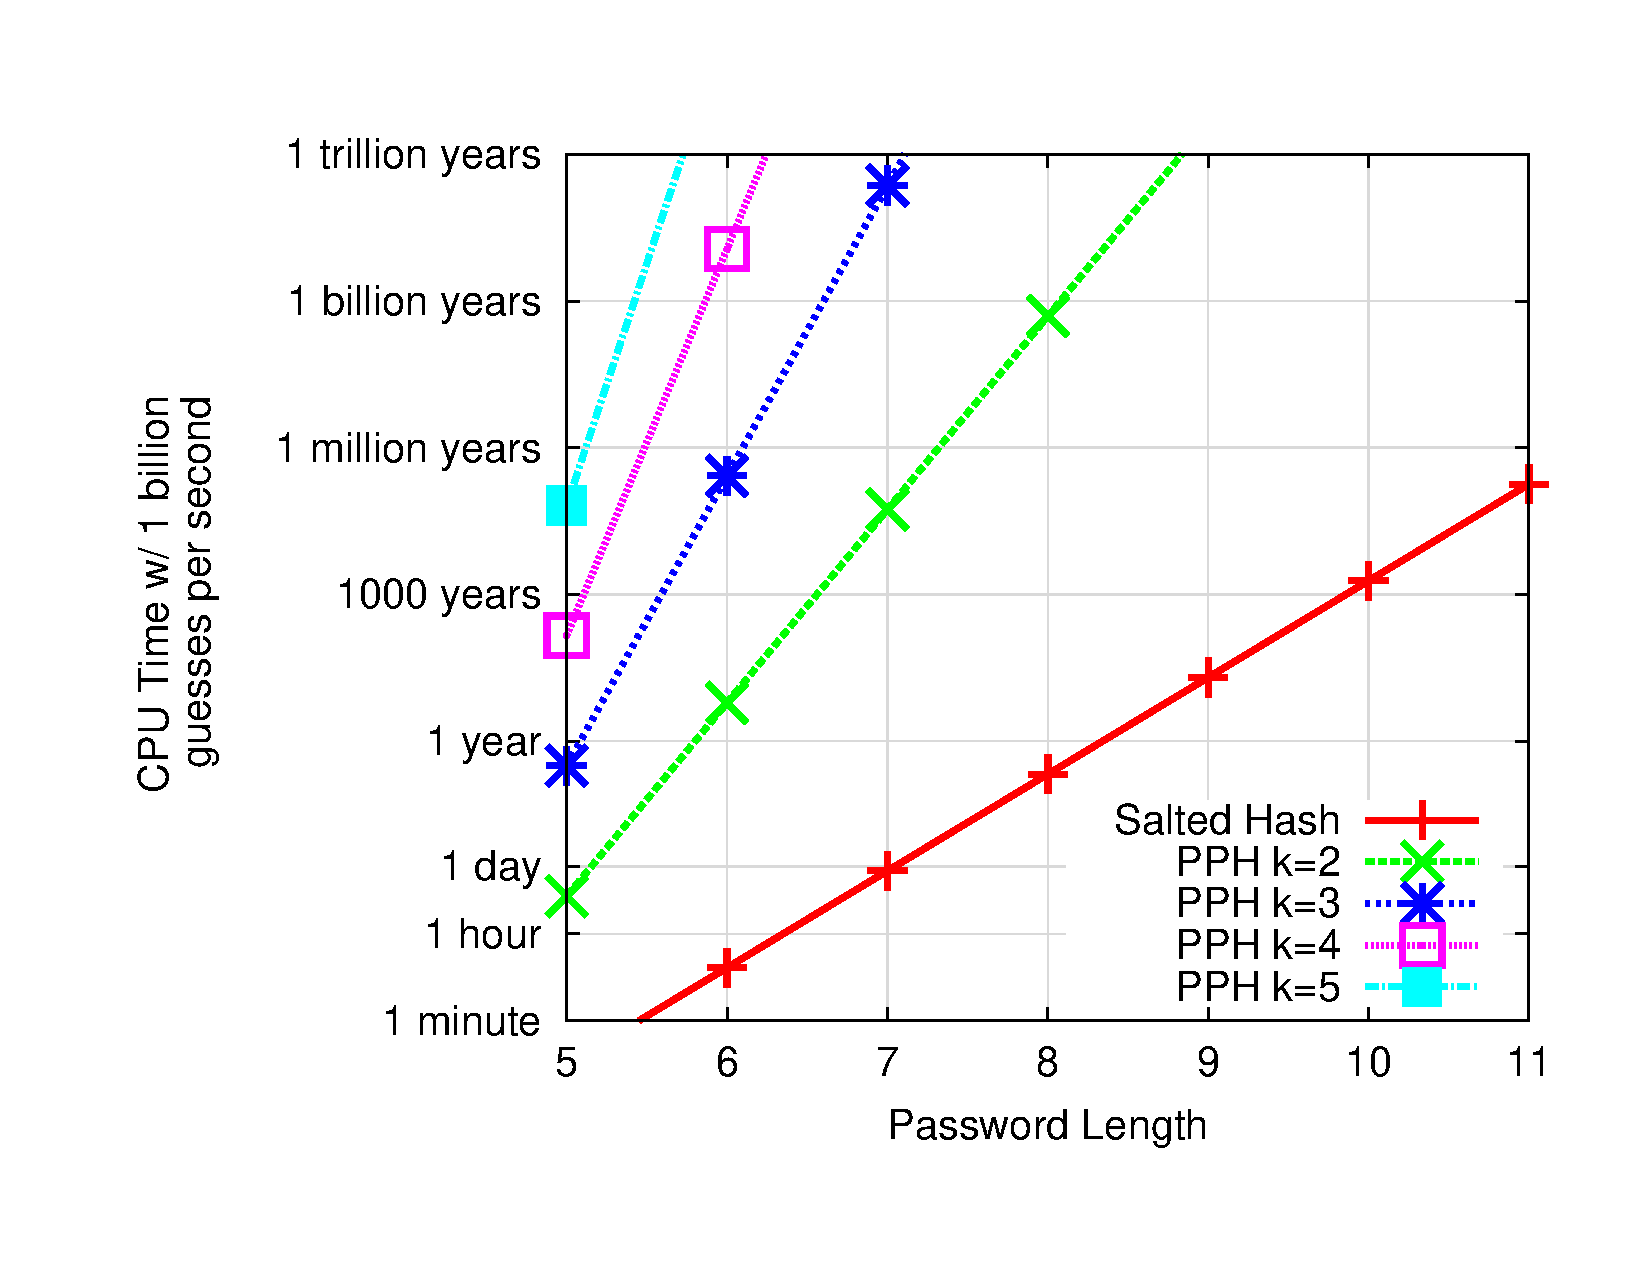
\includegraphics[width=.5\linewidth, trim=195 55 165 55]{./images/plotcrack_threshold}
    \caption{{\small Time it takes to crack a \PPH store with different values of 
    threshold and 24 \partialbytes}}
    \label{FIGURE:cracking-threshold}
\end{figure}

\subsection{What if a poor value is chosen for the threshold?}

Choosing a poor threshold setting can minimize the protections of \PPH.
If the threshold is too high, the system will primarily be in the 
bootstrapping phase while waiting for \thresholdaccounts to log in.  
Thus most of the accounts will be bootstrap accounts and only be protected 
by salted hashes.  If an attacker steals this database, they can individually 
crack these passwords.

An organization might find that there are not enough \thresholdaccount logins to get
the system into normal operation.   One way to mitigate this is to promote 
some \thresholdlessaccounts that log in frequently to be \thresholdaccounts.  
This would allow an attacker who controls one or more of those accounts to
have an easier time cracking the \thresholdaccounts, but causes bootstrapping
accounts to be protected.

{\bf Recommendation 7: It is often better to have \thresholdaccounts that 
frequently log in (but who are untrusted), than those of trusted users
who rarely log in.} 

If the threshold setting is too low, then an attacker can feasibly crack
the \thresholdaccounts and gain the ability to individually crack accounts.
This is particularly problematic when combined with a large \partialbytes
settion.  The minimum threshold setting described in the previous
settings should be used wherever possible. This relationship can be verified 
by consulting Table~\ref{TABLE:pph-configurations}



%\cappos{I'm of the opinion we should cut the Sony Breach.  Given time, we 
%could do an analysis of the RockYou database with the passwords that pass our
%filters.   (Entropy eval then look at this.)
%
%I don't think this helps our case and the argument about why we don't toss
%things is muddied by our other arguments...
%}

\eat{
\subsection{Case study: the Sony Breach}
\label{SUBSEC:sony-database}

To explore how these results carry over to real passwords, we performed an
experiment using the password data dumped from the Sony account
breaches~\cite{sonyhack}.  Of the leaked password databases known to the 
authors (Table~\ref{TABLE:disk-space}), this is the only data set which 
explicitly lists which accounts are administrator accounts versus normal users.

\santiago{this should be revised, what if we throw away the weak passwords}
In the database dump, there is password data for both outside user accounts as
well as accounts have administrator access. The four administrator accounts
have passwords with the estimated entropy in bits~\cite{passwordstrength}:
password@1 (5.322 bits), welkom@1 (26.553 bits), waderobsen (30.618 bits), and
itsafullcyrcle (44.011 bits). Given a rate of a billion password hashes checked
per second, the first three passwords can all be cracked in two seconds. The
remaining password (and thus every administrator password) could be cracked in
under 5 hours.

If \PPH were protecting these passwords, the ability to crack the
passwords would depend on the threshold. The effective password strength is
that of the weakest passwords combined, times the probability of selecting
those accounts in that order. A threshold of 3 will have an effective entropy
of 67.078 bits, which will take nearly 5000 years to crack, based on 1 billion
guesses per second.

With a threshold of 2, the effective entropy is 35.459 bits, which can be
cracked in under a minute. However, if all administrators chose a password as
strong as the password waderobsen (which is considered a weak password by
current standards~\cite{passwordstrength}), then the password would have had an
effective entropy of 64.820 bits, and take more than a thousand CPU years to
crack at 1 billion guesses per second. This underscores the fact that
administrators still should not choose immensely poor passwords (e.g.,
‘password@1’).  Independent of password storage concerns, avoiding trivially
guessable passwords is essential in preventing remote brute-force password
cracking.

\Thresholdlessaccount passwords (many of which tend to be extremely weak) cannot
be cracked until a threshold of administrator passwords are compromised. This
means that even it is only administrators who can be convinced to use strong
passwords, \PPH still provides substantial security benefits.


\eat{
\santiago{This is part of the old eval, we can take information from here}
\Partialverification allows an attacker to first reduce the search space for a
specific account by eliminating accounts that do not match the leaked bits. If
the attacker knows the password pattern, he can first precompute all passwords
that match that pattern and hash. This requires the same amount of effort
(k*2n) as for cracking passwords that are stored using traditional best
practices. If the attacker has sufficient space to store these passwords, he or
she may then use combinations of these precomputed passwords to try to unlock
the database. The attacker will be able to search the space for the Shamir
Secret Store in 2k*n-l guesses.  Each byte used for \partialverification
effectively reduces the strength of a random password by approximately 1.22
characters. However, the time needed to unlock the Shamir Secret Share still
represents an exponential increase and dominates the overall cost.

With one billion operations per second, sweeping the search space would still
require 45 thousand CPU years (8 orders of magnitude more time than salting and
hashing).  For example, if 2 bytes are leaked for 6 random character passwords
(Figure~\ref{FIGURE:cracking-times}), the attacker will need to do 735 trillion
operations for each of the three passwords and then 1.41×1021 operations to
crack the password database. 
}
\subsection{Summary}
\label{SUBSEC:summary}
}

\section{Related Work}
\label{SEC:related-work}

Given the ubiquity of passwords, password security has become an important
research area in both academia and industry. Hackers have also found password
databases enticing and have devoted time and resources to figuring out new
strategies for gaining access to passwords and associated user identities.
Hackers’ persistence in developing ever more sophisticated cracking strategies
has in turn focused researchers, who have come up with many promising solutions
that each solve different portions of the problem.

In this section, we categorize related work according to their requirements
for deployment. Solutions that 
use additional server hardware or servers require effort to deploy but tend 
to present very strong protection.  Changes that involve the client also
require effort to deploy (on clients), but in many cases are also very
effective at protecting user information. There are relatively
few solutions that only require changes on the server side and are software
only.  However, these solutions, like salted hashing and key stretching,
tend to be very widely deployed.  \PPH is the first solution of this
type that increases attackers' cracking effort asymmetrically more
than the increase to the server's verification time.
%\begin{itemize}
%    \item Assumes the attacker can read all persistent storage
%
%    \item Requires only a software change on the server
%
%    \item Requires exponentially more time for the attacker to be able to crack
%    passwords
%
%\end{itemize}
%
%In this subsection, we enumerate different password storage mechanisms organized
%by their threat model and how it relates to the threat model of \PPH.
%
%\linda{LV: I think there needs to be some sort of lead in to the rest of this
%section -- most likely would be to set up organizing this section around threat
%models...}

\eat{
\begin{table}[b]

    \centering
    \renewcommand{\arraystretch}{1.3}
    \caption{Different authentication mechanisms and their security features}
    \label{TABLE:authentication-technologies}

    \centering
    \begin{tabular}{| c | c | c | c |}
    \hline
    {\bf Auth.} & {\bf Changes to} & {\bf Extra} & {\bf Memory} \\
    {\bf mechanism} & {\bf client} & {\bf Hardware} & {\bf safe} \\
    \hline
    Multi-server & No & Yes & N/A \\
    \hline
    Decoys & No & Yes & No \\
    \hline
    Key Stretching & No & No & No \\
    \hline 
    Biometrics &  Yes & Yes & No/Yes \\
    \hline
    \end{tabular}
\end{table}
}

\subsection{Systems that Require Extra Servers or Server-side Hardware}

{\bf Multi-server Password Authentication.} A wide variety of
authentication schemes use multiple servers to store password
data~\cite{Chai20071046, bagherzandi2011password, katz2005two}. The assumption
is that an attacker cannot compromise a threshold of the servers. In contrast,
\PPH uses a threshold system to hide information in memory on a single server 
that can only be unlocked with a threshold of correct user passwords.

Prior work by Gwoboa~\cite{gwoboa1995password} hides passwords using
a trapdoor function (public key cryptography) and techniques from threshold
cryptography.   It can authenticate users with two hidden pieces of 
information, a user ID (likely not the user name, for security reasons) and 
the password.   However, a major concern of the scheme is how the private
key is stored on the server.   The authors propose splitting it amongst 
multiple systems and using threshold cryptography.   %Clearly if all 
%persisted data is known, this key (and thus all passwords) are at risk.
%In \PPH, as long as a threshold of passwords are not known, all 
%persisted data can be stolen by an attacker without compromising user 
%passwords.


{\bf Decoys.}  Recently, researchers have suggested an array of techniques
that employ sets of extra password entries~\cite{Kontaxis_CCS_2013,
juels2013honeywords}.  For example, the
Honeywords~\cite{juels2013honeywords}system uses a separate server to hold
information that authenticates the correct password entry. Once attackers
obtain a password database they do not know which password entry is correct.
Entering a password that matches a hash to the wrong password entry will
trigger an alarm that notifies the administrator that there has been a password
hash file breach.  However, for this to work, there must be a separate, secure
server to authenticate the index of that entry (a one byte value).  An 
important attribute of HoneyWords is that it can also operate when the 
server is offline and will check passwords and detect breaches when the 
server comes back online.  
This is similar to the way that accounts validated during bootstrapping in
\PPH are re-validated after a threshold of \thresholdaccount passwords are
provided.

{\bf Using a hardware database encryption key.} Storing a key in trusted
hardware (such as a USB dongle~\cite{passwordhardwaredongle}) has security benefits, but also has
deployment challenges. If the hardware stops working, the protected
data is likely to be irrevocably lost. To have backup servers, it is essential
to have identical duplicate copies of the secure token. This complicates use in
scenarios like cloud computing or even just a standard master / slave
deployment. %On the other hand, \PPH is entirely software based
%and a backup system can be brought online in the same way that a normal server
%boots.  \cappos{integrate into above}\santiago{Maybe it doesn't fit here
%anymore}


{\bf Bounded Attacker.} Di Crescenzo~\cite{di2006perfectly} proposed a
scheme for protecting password data when an attacker can only read a bounded
amount of data from storage.   This entails that an organization configure
network monitoring hardware and set up a separate server to process
authentication requests.  %In the widely published password file compromises,
%the attackers were able to steal complete password file
%data~\cite{miranteTR13,passwordresearchblog}.   In contrast, \PPH
%requires no network changes or monitoring and works even when an attacker has
%complete access to stored information, such as a disk backup.
This may pose a deployment challenge for some organizations.

{\bf Single Sign-On.} Single sign-on systems such as OpenID and OAuth have
promise for organizations to securely offload authentication to a third party.
This is convenient for users, but is far from ubiquitous for a variety of
reasons~\cite{sun2010billion}. Single sign-on systems have known security
issues~\cite{openidsecurity, oauthsecurity}, but overall can be effective 
when properly used. \PPH integrates cleanly with such systems
and can trivially allow \thresholdlessaccounts to verify with them. In 
addition, \PPH could be used by a Single Sign-On
provider to securely store its password database.



\subsection{Systems That Require Client Side Changes}

{\bf Biometrics.} Biometric authentication is a promising field for secure
password authentication~\cite{atallah2005secure, snelick2005large,
tuyls2004capacity, boyen2005secure, erkin2009privacy, kerschbaum2004private,
osadchy2010scifi, monrose2001cryptographic, sae2012biometric}, with a
substantial amount of work already done on how to store and authenticate users
with biometric information. Like \PPH, some of these approaches
use a threshold system to validate and authenticate users, in part to deal with
noisy biometric data~\cite{juels2006fuzzy, ballard2008practical}.  Although
\PPH also requires users to remember a password, it does not
require client-side hardware.  Moreover, prior work uses keystroke dynamics to
change stored password data~\cite{monrose2000keystroke} and relies on reading timing information
as users type their passwords during login. This method of analyzing
timing of keystrokes 
provides promising protections, but requires changes to the client and server
to correctly operate. 
%In comparison, \PPH protects password hash
%information with no changes to the client and minimal server changes.

{\bf Authentication Using Tokens or Smart Cards.} Much investigation has
looked at authentication systems. These systems, which use
hardware tokens, are popular in banking~\cite{deo1998authentication,
yeh2010two}, health services~\cite{ahn2002towards}, as well as in more general
contexts~\cite{chien2002efficient, yang1999password}. These systems are
extremely effective and are widely used to limit and protect access to
classified systems, often by integrating a threshold cryptosystem to provide
multifactor authentication using hardware tokens~\cite{brush2014pico, yubikeyhardware}.
There are even client devices that one can use either as a primary
authentication source or as a second factor of authentication.


%Unfortunately, these devices incur a per-user cost and are not widely
%deployed yet.
%thus are not often used in contexts where the
%user and server have no prior commercial or authentication relationship. In
%contrast, \PPH can be used in webmail systems and social networks
%where this relationship does not exist a priori -- a running system with regular
%salted-hash storage can easily upgrade to \PPH without affecting
%a user’s login procedure in any way.

{\bf Password Managers.} There are a myriad of password managers that help
users choose and manage secure per-site passwords including LastPass,
1Password, and OnePass. These systems store password data and lock it with the
user's credentials. However, these third party software  (and often their
servers) will know users' passwords, which opens the door to potential
misuse.  To mitigate this, several groups have proposed cryptographic
techniques that will similarly take a user's password and generate secure, per
site passwords~\cite{halderman2009lest,ross2005stronger,
halderman2005convenient}. These techniques are effective (and more secure) but
can create passwords that are incompatible with a server's password policy.
Password manager tools require client-side changes or support, whereas
\PPH requires server-side changes only. Both can be used in
conjunction safely for improved security.

{\bf Multiparty Computational Authentication.} There are a variety of
schemes that perform secure, remote authentication using computation by the
client and server on legacy hardware~\cite{wu1998secure, Lomas_SOSP_89,
chien2001modified, jan1998paramita, gong1995optimal,
camenisch2010credential, brainard2003nightingale, katz2001efficient,
katz2003forward, gong1993protecting}. These schemes have significant, positive
aspects such as (in some cases) requiring an attacker to be online to validate
communications. However, they require multiparty protocols that require changes
on clients and servers. %They also do not function in non-distributed scenarios.
%\PPH works with no changes to clients, minimal visible changes to
%the administrator, and operates on a single system.

{\bf Non-password Authentication.} Many researchers have proposed
authentication based upon non-password items such as
pictures~\cite{dhamija2000deja}. In practice, these systems can face security
limitations if users do not appropriately choose their authentication
tokens~\cite{davis2004user}.  Used with these authentication mechanisms, 
\PPH functions well
for \thresholdlessaccounts, requiring no changes to the system.  However, 
unless a key or hash can be derived from such mechanisms, it may not
be possible to use them to recover a \thresholdaccount's share.


{\bf Key Exchange Schemes.} There are also many systems that
implement secure key exchange~\cite{shoup1999formal}, such as Password
Authenticated Key Exchange (PAKE)~\cite{boyko2000provably,
shen2010towards,sathik2010secret, jablon1996strong}, Encrypted Key Exchange
(EKE)~\cite{steiner1995refinement, lucks1998open, jablon1997extended}, and
further enhancements~\cite{wang2005strengthening}. These systems allow parties
who share a password to securely find an encryption key to hide their
communications. These systems provide excellent protection and can handle
compromises to a system's memory, in many cases. However, unlike
\PPH, they typically involve multi-round authentications and
require changes to both the client and server.

{\bf Helping Users Choose Stronger Passwords.} There have been many
efforts to help users choose stronger, more memorable passwords and understand
what constitutes a weak
password~\cite{topkara2007passwords,klein1990foiling,bishop1995improving,
schechter2010popularity, komanduri2011passwords, shay2010encountering,
xkcdpassword}. Such efforts could be quite effective in protecting users, but
users will need to adopt new password habits and strategies.
%\PPH provides an exponential improvement in protection for user
%passwords.  
We leverage studies by~\cite{weir2010passwordpolicies, cormac2007passwordhabits,
cormac2014telepathwords, kelley2012guessingpasswords} to understand how
to add policies that improve entropy in \thresholdaccount passwords.

{\bf Two-Factor Authentication.} The use of two-factor
authentication~\cite{di2005two} is provided by some popular services (typically
through an SMS or phone call).  Two-factor authentication does not change
\PPH's use in any way.  Users can easily get the best of both
protections with simultaneous deployment of each technology.

\subsection{Server-Side, Software-Only}

These mechanisms fall directly into the same threat model as \PPH. 


{\bf Key Stretching.} One way to mitigate the effectiveness of cracking
salted hashes is to use key stretching techniques~\cite{kelsey1998secure}. This
involves performing multiple rounds of cryptographic operations to validate a
hash (or key).  But key stretching incurs a slowdown for the attacker, 
proportional to the number of iterations.  Unfortunately, it also slows the
server down by the same factor, which limits the effectiveness of the 
technique.

\PPH leverages key stretching in two parts of the algorithm in a way
that poses a much higher cost to the attacker than the server.  
\PPH may also use key stretching during \partialverification.  This
increases the authentication time only when bootstrapping, yet increases the time cost 
to the attacker for all cracking efforts. When the server
is in normal operation, there is no slowdown.  This presents an increase
that is the same factor for the server and attacker, but the server only
needs to pay the cost for a short period.  

The more impactful use of key stretching is when \PPH performs an integrity 
check on the secret before transitioning to normal operation.  This operation 
is done only once per reboot by the server, yet the attacker must perform
this operation once per guess of \thresholdaccount passwords.   This causes 
an enormous, asymmetric increase in cracking time for the attacker.


\eat{
\PPH implements key stretching for \partialverification
in order to slow down attackers who attempt to crack the isolated-check bits
field. Yet,   \santiago{We can mention stretching on the
secret verification hash}
}

\eat{
\santiago{This doesn't seem to fit here}
Using \partialverification, \PPH can process user authentications
immediately, without the security risks associated with administrator shared
keys. With \PPH, administrators do not need to share passwords or
keys. Each administrator will have their own password; this allows access and
system administration to go on even as administrators join and leave the
organization. 
}

\section{Conclusion}
\label{SEC:conclusion}

This work presents \PPH, a technique for protecting user passwords in the 
event of password database disclosure. \PPH is the first technique
that requires only software changes on the server and yet requires
attackers to do asymmetrically more work to crack passwords than
servers need to do to verify them.  As a result, password
cracking becomes infeasible for attackers in many cases.


\PPH is practical to deploy and is effective in practice.  The performance
of \PPH is similar to salted hashing.  The memory and storage costs from
using \PPH are negligible.  So long as good password selection procedures
are followed, \thresholdaccounts increase an attacker's cracking effort by
many orders of magnitude.  We show how configuring \partialverification
in different ways can help to optimize \PPH for different configurations
of services.

We have installed \PPH at our institution and are gaining practical
experience to uncover any usability problems.  Five different parties, 
two of whom had no prior contact with us, authored an implementation
of \PPH.  There are implementations for a variety of languages and 
web frameworks available with an MIT license at:
\showurlx. 





\dmyyyydate
%   {\footnotesize \bibliographystyle{acm}
%   \bibliography{bibdata}}
\bibliographystyle{IEEEtran}
\bibliography{IEEEabrv,bibdata}
% \theendnotes

\end{document}
